% documentclass options:
% ngerman is needed for hyphenation if the thesis contains parts written in German
% BCOR is binding correction
% if you'd rather have a one sided thesis, add `onside' to the documentclass
\documentclass[12pt, a4paper, BCOR=10mm, english, ngerman, oneside]{scrbook}

% include all packages and define commands in setup.tex
%--------
%       package includes
%--------
    % font encoding is set up for pdflatex, for other environments see
    % http://tex.stackexchange.com/questions/44694/fontenc-vs-inputenc
    \usepackage[T1]{fontenc}  % 8-bit fonts, improves handling of hyphenations
    \usepackage[utf8x]{inputenc}
    % provides `old' commands for table of contents. Eases the ability to switch between book and scrbook
    \usepackage{scrhack}
    \usepackage{parskip}

    % ------------------- layout, default -------------------
    % adjust the style of float's captions, separated from text to improve readabilty
    \usepackage[labelfont=bf, labelsep=colon, format=hang, textfont=singlespacing, font=small]{caption}
    
    \usepackage{chngcntr}  % continuous numbering of figures/tables over chapters
    \counterwithout{equation}{chapter}
    \counterwithout{figure}{chapter}
    \counterwithout{table}{chapter}

    % Uncomment the following line if you switch from scrbook to book and comment the setkomafont line
    %\usepackage{titlesec}  % remove "Chapter" from the chapter title
    %\titleformat{\chapter}[hang]{\bfseries\huge}{\thechapter}{2pc}{\huge}
    \setkomafont{chapter}{\normalfont\bfseries\huge}

    \usepackage{setspace}  % Line spacing
    \onehalfspacing
    % \doublespacing  % uncomment for double spacing, e.g. for annotations in correction

    % ------------------- functional,default-------------------
    \usepackage[dvipsnames]{xcolor}  % more colors
    \usepackage{array}  % custom format per column in table - needed on the title page
    \usepackage{graphicx}  % include graphics
    \usepackage{subfig}  % divide figure, e.g. 1(a), 1(b)...
    \usepackage{amsmath}  % |
    \usepackage{amsthm}   % | math, bmatrix etc
    \usepackage{amsfonts} % |
    \usepackage{calc}  % calculate within LaTeX
    \usepackage{algorithm,algpseudocode}
    \usepackage[unicode=true,bookmarks=true,bookmarksnumbered=true,
                bookmarksopen=true,bookmarksopenlevel=1,breaklinks=false,
                pdfborder={0 0 0},backref=false,colorlinks=false]{hyperref}
    \usepackage{hyperref}
    \usepackage[nameinlink,noabbrev]{cleveref}
    \usepackage{wrapfig}
    \usepackage{acronym}
    \usepackage{fancyhdr}
    \fancyhf{}
    \fancyhead[RE,RO]{ \rightmark}
    \fancyfoot[CO,CE] {\thepage}

\usepackage{tabularx}

\renewcommand{\figurename}{Abbildung}
\renewcommand{\contentsname}{Inhaltsverzeichnis}
\renewcommand{\tablename}{Tabelle}
\renewcommand{\bibname}{Literaturverzeichnis}
\renewcommand{\chaptername}{Kapitel}
\renewcommand{\listfigurename}{Abbildungsverzeichnis}

    %==========================================
    % You might not need the following packages, I only included them as they
    % are needed for the example floats
    % ------------------- functional, custom-------------------

    \usepackage{bm}  % bold greek variables (boldmath)
    \usepackage{tikz}
    \usetikzlibrary{positioning}  % use: above left of, etc

    % Improves general appearance of the text
    \usepackage[protrusion=true,expansion=true, kerning]{microtype}

    \usepackage[graphicx]{realboxes}
    \usepackage{adjustbox}

%------- (re)new commands / settings
    % ----------------- referencing ----------------
    \newcommand{\secref}[1]{Section~\ref{#1}}
    \newcommand{\chapref}[1]{Chapter~\ref{#1}}
    \renewcommand{\eqref}[1]{Equation~(\ref{#1})}
    \newcommand{\figref}[1]{Figure~\ref{#1}}
    \newcommand{\tabref}[1]{Table~\ref{#1}}

    % ------------------- colors -------------------
    \definecolor{darkgreen}{rgb}{0.0, 0.5, 0.0}
    % Colors of the Albert Ludwigs University as in
    % https://www.zuv.uni-freiburg.de/service/cd/cd-manual/farbwelt
    \definecolor{UniBlue}{RGB}{0, 74, 153}
    \definecolor{UniRed}{RGB}{193, 0, 42}
    \definecolor{UniGrey}{RGB}{154, 155, 156}


    % ------------------- layout -------------------
    % prevents floating objects from being placed ahead of their section
    \let\mySection\section\renewcommand{\section}{\suppressfloats[t]\mySection}
    \let\mySubSection\subsection\renewcommand{\subsection}{\suppressfloats[t]\mySubSection}


    % ------------------- marker commands -------------------
    % ToDo command
    \newcommand{\todo}[1]{\textbf{\textcolor{red}{(TODO: #1)}}}
    \newcommand{\extend}[1]{\textbf{\textcolor{darkgreen}{(EXTEND: #1)}}}
    % Lighter color to note down quick drafts
    \newcommand{\draft}[1]{\textbf{\textcolor{NavyBlue}{(DRAFT: #1)}}}


    % ------------------- math formatting commands
    % define vectors to be bold instead of using an arrow
    \renewcommand{\vec}[1]{\mathbf{#1}}
    \newcommand{\mat}[1]{\mathbf{#1}}
    % tag equation with name
    \newcommand{\eqname}[1]{\tag*{#1}}


    % ------------------- pdf settings -------------------
    % ADAPT THIS
    \hypersetup{pdftitle={KarinaSchmunkBSC},
                pdfauthor={Karina Schmunk},
                pdfsubject={Bachelorarbeit an der Fachhochschole Aachen},
                pdfkeywords={process mining, smart living,  computer science},
                pdfpagelayout=OneColumn, pdfnewwindow=true, pdfstartview=XYZ, plainpages=true}


    %==========================================
    % You might not need the following commands, I only included them as they
    % are needed for the example floats

    % ------------------- Tikz styles -------------------
    \tikzset{>=latex}  % arrow style


    % ------------------- algorithm ---------------------
    % Command to align comments in algorithm
    \newcommand{\alignedComment}[1]{\Comment{\parbox[t]{.35\linewidth}{#1}}}
    % define a foreach command in algorithms
    \algnewcommand\algorithmicforeach{\textbf{foreach}}
    \algdef{S}[FOR]{ForEach}[1]{\algorithmicforeach\ #1\ \algorithmicdo}

%___________________________________________________________
\usepackage{listings}

\usepackage{color}
\definecolor{gray}{rgb}{0.4,0.4,0.4}
\definecolor{darkblue}{rgb}{0.0,0.0,0.6}
\definecolor{cyan}{rgb}{0.0,0.6,0.6}

\definecolor{pblue}{rgb}{0.13,0.13,1}
\definecolor{pgreen}{rgb}{0,0.5,0}
\definecolor{pred}{rgb}{0.9,0,0}
\definecolor{pgrey}{rgb}{0.46,0.45,0.48}


\lstset{
  basicstyle=\fontsize{9}{11}\selectfont\ttfamily,
  columns=fullflexible,
  showstringspaces=false,
  commentstyle=\color{gray}\upshape
}

\lstdefinelanguage{XML}
{
  morestring=[b]",
  morestring=[s]{>}{<},
  morecomment=[s]{<?}{?>},
  stringstyle=\color{black},
  identifierstyle=\color{darkblue},
  keywordstyle=\color{cyan},
  morekeywords={xmlns,version,type,value,key}% list your attributes here
}

\lstset{language=Java,
  showspaces=false,
  showtabs=false,
  breaklines=true,
  showstringspaces=false,
  breakatwhitespace=true,
  commentstyle=\color{pgreen},
  keywordstyle=\color{pblue},
  stringstyle=\color{pred},
  basicstyle=\ttfamily,
  moredelim=[il][\textcolor{pgrey}],
  moredelim=[is][\textcolor{pgrey}]
}

\begin{document}
    \pagestyle{empty} % no header and no page number
    % disable hyper links to remove warning "destination with same identifier"
    % this means within this section nothing can be referenced with a hyperlink
    \hypersetup{pageanchor=false}
    \begin{titlepage}
\begin{center}
\hfill

\includegraphics[width = 14mm]{figures/Appbildungen/FHAachen-logo.png}
\newcommand{\HorizontalLine}{\rule{\linewidth}{0.3mm}}
% _____________________________________________________________________________
%\HorizontalLine \\[0.4cm]
\begin{spacing}{2.5}
    \textsc{\Large  Process Mining im Smart Living} \\
    \textsc{\Large  Szenario - Vergleich von Algorithmen} \\
    \textsc{\Large   unter dem Aspekt der Einbindung in einer If This Than That Anwendung}\\
\end{spacing}
\vspace{20mm}
%\HorizontalLine \\[0.5cm]
% _____________________________________________________________________________

{\Large \bfseries Bachelorarbeit}\\[1.1cm]
{\Large Verfasser: Karina Schmunk} \\[1.2cm]

\begin{tabular}[hc]{>{\large}l >{\large}l}
  \bfseries Erstprüfer: & Prof. Martin R. Wolf \\[0.3cm]
  \bfseries Zweitprüfer: & Prof. Matthias Mehring \\[1.2cm]
\end{tabular}
\vfill  % move the following text to the bottom

\Large {
    Fachhochschule Aachen\\
    Fachbereich Elektrotechnik und Informationstechnik\\
    Labor für IT Organisation und Management\\[1cm]

    
}
\end{center}
\end{titlepage}

    \pagestyle{plain} % remove chapter name from top, page number at the bottom
    \frontmatter  % roman page numbers
    \chapter*{Kurzbeschreibung}\vspace{17mm}
Die vorliegende Bachelorarbeit hat die Eignung von Process Mining Algorithmen für den Einsatz in Smart Living Szenarien zum Thema. Hierfür werden die gängigsten Process Mining Algorithmen in einer Testreihe miteinander verglichen und daraufhin untersucht, ob sie sich zur Vorhersage von repetitivem menschlichen Verhalten eignen, das durch vernetzte Geräte im Haushalt aufgezeichnet wurde. Als Proof of Concept wird eine Vorhersagefunktion in eine Android-Anwendung integriert, die einem Anwender Vorschläge in der sogenannten If This Then That Form, basierend auf den Ergebnissen eines Process Mining Algorithmus, unterbreitet und in der Lage ist, diese Regel selbstständig im Smart Home System zu hinterlegen. Für die automatisierte Regelerkennung wird ein Skript umgesetzt, das die Durchführung der Analyse in einem lokalen Netzwerk und mit geringem Rechenressourcenverbrauch erlaubt.

Ziel einer solchen Anwendung ist die Erleichterung des Umgangs mit der wachsenden Anzahl vernetzter Geräte im privaten Raum, indem der Verbraucherin oder dem Verbraucher Konfigurationsschritte durch intelligente Analyse abgenommen werden, ohne dass dabei private Daten an Dritte gelangen.

Die Ergebnisse der Testreihe deuten darauf hin, dass das Heuristic Miner Verfahren geeignet ist, gesuchte Prozesse derart zu modellieren, dass sie in eine Regel überführt werden können, die dann das Potential hat, den Komfort der Bewohnerin oder des Bewohners eines Smart Homes zu erhöhen.

\newpage
\chapter*{Abstract}\vspace{17mm}
The aim of this thesis is to examine the suitability of process mining algorithms for use in smart living scenarios. For this purpose, the most common process mining algorithms are compared with each other in a test series and examined as to whether they are suitable for predicting repetitive human behavior, which is  recorded by IoT devices in the household. As a proof of concept, a prediction function is integrated into an Android application, which makes suggestions to the user in the so-called If This Then That Form, based on the results of a process mining algorithm. 
For automated rule recognition, a script is implemented that allows the process mining analysis to be performed in a local network, requiering only low computing resources. 

The aim of such an application is to facilitate the handling of the growing number of networked devices in private spaces. This is achieved by removing configuration steps from the consumer through intelligent analysis, without private data being passed on to third parties. 

The results of the test series indicate that the Heuristics Miner method is suitable for modelling short patterns of human behavior in such a way that they can be converted into. This, in turn, has the potential to increase the comfort of the occupant of a smart home.

    \chapter*{Abschlusserklärung}
 \thispagestyle{empty}

Ich versichere hiermit, dass ich die vorliegende Arbeit selbständig verfasst und keine anderen als die im Literaturverzeichnis angegebenen Quellen benutzt habe.
Stellen, die wörtlich oder sinngemäß aus veröffentlichten oder noch nicht veröffentlichten Quellen entnommen sind, sind als solche kenntlich gemacht.
Die Zeichnungen oder Abbildungen in dieser Arbeit sind von mir selbst erstellt worden oder mit einem entsprechenden Quellennachweis versehen.
Diese Arbeit ist in gleicher oder ähnlicher Form noch bei keiner anderen Prüfungsbehörde eingereicht worden.
\\[3\normalbaselineskip]
\begin{tabular}{p{\textwidth/2} l}
  \rule{\textwidth/3}{0.4pt}   &   \rule{\textwidth/3}{0.4pt} \\
  Aachen, den                  &   Unterschrift
  \\
                               &   (Schmunk, Karina)
\end{tabular}
\newpage
\subsubsection{Genderhinweis}
\normalsize{
Aus Gründen der besseren Lesbarkeit wird in dieser Bachelorarbeit die Sprachform des generischen Maskulinums  angewandt.  Es  wird  an  dieser  Stelle  darauf  hingewiesen,  dass  die  ausschließliche Verwendung der männlichen Form geschlechtsunabhängig verstanden werden soll.}
    \tableofcontents
    \listoffigures
    \listoftables
   % \listofalgorithms
    \hypersetup{pageanchor=true}  % re-enable hyperlinking

    \mainmatter  % Arabic page numbers
    \pagestyle{fancy}
%    \documentclass{article}
\usepackage[nohyperlinks, printonlyused, withpage, smaller]{acronym}

\begin{document}

\section*{Abkürzungsverzeichnis}

\begin{acronym}[ECU]
\acro{ecu}[ECU]{European currency unit}

\end{acronym}

\end{document}
    \chapter{Einleitung}\label{chap:introduction}
Mit einem wachsenden Angebot an Smart Home Geräten auf dem Weltmarkt nimmt auch die Anzahl der Plattformen stetig zu, die Lösungen für die Steuerung von vernetzten Geräten anbieten. Mit dieser wachsenden Vielfalt erhöht sich auch der Bedarf an benutzerfreundlichen Schnittstellen für die Kommunikation mit dem intelligenten Eigenheim. Dass das Smart Home zunehmend an Relevanz gewinnt und zukünftig allgegenwärtig sein wird belegen unter anderem die Zahlen des Marktforschungsunternehmens IDC. Das Wachstum des weltweiten Smart Home Markts im Jahr 2019 wird auf voraussichtlich 26,9 \% und 832,7 Millionen verkaufte Geräte geschätzt \cite{IDC}.
 
Einer breiten Adaption von intelligenter Haustechnik stehen gegenwärtig noch einige Vorbehalte der Nutzer entgegen. Hemmnisse für die Akzeptanz von Smart Home Systemen betreffen vordergründig Bedenken hinsichtlich des Datenschutzes und der Datensicherheit, so die Herausgeber einer Studie des Marktforschungsinstituts Dr. Grieger \& Cie \cite{griegercie}. Das IDC hält auch in Anbetracht der Bedenken seitens der Verbraucher an einer positiven Marktprognose fest, was durch Aussagen der Befragten begründet wird, wonach der Zugewinn an Komfort durch Smart Home Geräte die Sorgen bezüglich der Datensicherheit häufig überwiege.
 
Um den Ansprüchen nach mehr Komfort gerecht zu werden, müssen intelligente Systeme nicht nur auf die vom Nutzer geäußerte Wünsche reagieren, sondern dessen Bedürfnisse antizipieren, so die Maxime von marktführenden Herstellern wie Amazon oder Google \cite{IoTGoogle}. Um dies zu ermöglichen werden IoT Geräte durch Verfahren aus den Forschungsfeldern der künstlichen Intelligenz und der Big Data Analyse gestützt, die eine Auswertung der gesammelten Daten über die Interaktion des Nutzers mit IoT Geräten erlauben und in der Lage sind Prognosen zur Nutzung der Geräte zu treffen. 
\newpage
Ein solches Verfahren, das dem Gebiet der Datenanalyse zuzuordnen ist, und seinen Ursprung unter Anderem in der Auswertung von Geräten in der maschinellen Produktion hat, ist das Process Mining. Process Mining ist ein Forschungsgebiet, das sowohl mit der Business Intelligence als auch mit Data Science Schnittmengen bildet \cite{PMinAction}. 

Es unterscheidet sich von konventionellem Data Mining insofern, als es sich vordergründig mit der Analyse von in der reellen Welt ablaufenden Prozessen beschäftigt. Es befasst sich nicht mit der Klassifizierung von Momentaufnahmen oder mit der Beantwortung von vergleichbaren instanzbezogenen Fragestellungen. Viele Technologien zur automatisierten Datenanalyse, wie etwa die Bilderkennung oder die linguistische Datenverarbeitung, beschäftigen sich mit Problemen, die unabhängig von einem zeitlichen Kontext zu betrachten sind. Anders verhält es sich beim Process Mining, dessen Hauptaugenmerk auf der sogenannten \textit{process awareness}, also dem Prozessbewusstsein, liegt.
\section{Fragestellung}
Ein Smart Home beschreibt ein System, das den Komfort im Eigenheim durch technische Lösungen erhöht, indem ein Netzwerk aus untereinander oder mit dem Nutzer interagierenden elektronischen Geräten im Gebäude integriert wird. Diese Geräte verfügen, neben ihrer inhärenten Funktionalität, auch über die Fähigkeit einen Logeintrag aus jeder ihrer Interaktionen oder Sensoraufnahmen zu generieren. Der Umstand, dass Process Mining Algorithmen zu erst Protokolldateien derjenigen Umgebungen benötigen, die sie analysieren sollen, legt die Kombination von Process Mining und dem System Smart Home nahe.
 
Bisher ist diese technologische Schnittstelle noch nicht tiefgreifend erforscht. Es sind nur vereinzelt Studien veröffentlicht worden, die die genannten Technologien miteinander kombinieren. Die vorliegende Arbeit soll klären, ob bestehende Process Mining Algorithmen in einem Smart Home effektiv eingesetzt werden können, um menschliches Verhalten korrekt zu abstrahieren. Ziel ist es dabei die Analyse kleiner Datensätze mit existierenden Softwarelösungen so zu gestalten, dass sie dem Benutzerkomfort im Umgang mit IoT Geräten zuträglich sind. Zweck der Architektur ist es die Auswertung gleichzeitig so ressourcenschonend aufzubauen, dass private Daten des Nutzers das lokale Netz nicht verlassen müssen.

\section{Zielsetzung}
Im Detail soll erarbeitet werden, ob Process Mining dazu eingesetzt werden kann, um menschliches Verhalten auf kurze, wiederkehrende Verhaltensmuster hin zu untersuchen und welches der gängigen Process Mining Verfahren für diesen Einsatzzweck besonders geeignet erscheint. Für eine Vorauswahl werden zunächst Studien betrachtet, die Process Mining bereits im Bereich des Smart Living eingesetzt haben. Anschließend werden diese systematisch in einer Testreihe miteinander verglichen, um festzustellen welche Leistungsfähigkeit von den etablierten Process Mining Algorithmen in dem darstellbaren Smart Living Szenario erwartet werden kann. Wichtige Kriterien sind dabei die Fehleranfälligkeit, die Rate vollständig akkurat erkannter Muster, sowie der Umgang mit Rauschdaten und parallel verlaufenden Prozessen.

Als Simulationsumgebung für den Einsatz des Programms soll ein Modell eines Smart Home dienen, das im Rahmen einer Bachelorarbeit am IT Institut für Organisation und Management der Fachhochschule Aachen entstanden ist und über die quelloffene Software openHab\footnote{https://www.openhab.org/docs/} gesteuert wird. Nach Auswertung der Protokolldateien nach unterschiedlichen Gesichtspunkten sollen die Erkenntnisse genutzt werden, um einen sogenannten Proof of Concept\footnote{Im Projektmanagement ist ein Proof of Concept, auch als Proof of Principle bezeichnet, ein Meilenstein, an dem die prinzipielle Durchführbarkeit eines Vorhabens belegt ist. In der Regel ist mit dem Proof of Concept meist die Entwicklung eines Prototyps verbunden, der die benötigte Kernfunktionalität aufweist.\cite{poc}} zu erstellen. Dieser wird auf einem einfachen Einplatinenrechner realisiert, der über eine Android App mit dem Anwender interagiert.

Ein Vorteil, den Process Mining dem Smart Home Anwender bieten kann, liegt in der automatisierten Erkennung von Prozessmustern im Umgang mit IoT Geräten. Bisher bieten eine Reihe von Unternehmen Plattformen an, die es dem Anwender lediglich durch manuelle Eingabe von Abläufen ermöglichen, Prozesse im Eigenheim zu automatisieren. Häufig findet dafür das sogenannte If This Then That Muster Anwendung, wie es beispielsweise in Webthings von Mozilla\footnote{IoT.mozilla.org},  oder Stringify\footnote{stringify.com} eingesetzt wird. 
\newpage
If This Then That beschreibt das Schema einer Regel, die aus Bedingungen bestehet, die jeweils vorkonfigurierte Aktionen auslösen. Diese müssen vom Anwender selbstständig als wiederkehrend erkannt und über eine Eingabemaske konfiguriert werden. Wird die Fähigkeit von Process Mining genutzt, Muster in aufgezeichneten Protokolldateien zu erkennen, bietet sich diese Methode an, um dem Anwender Konfigurationen in seinem Smart Home automatisch vorzuschlagen. Er kann dann die vorgeschlagene Regel bestätigen oder ablehnen. Zum einen hätte diese Funktion den Vorteil, dass es weniger Konfigurationsaufwand seitens des Anwenders bedarf, um einen neuen automatisierten Ablauf in seinem Smart Home zu integrieren. Zum anderen ist es so möglich, dass ein Algorithmus Muster erkennt, die der Aufmerksamkeit des Anwenders entgangen wären, aber durch eine Implementierung den Komfort im Smart Home erhöhen.

%Die Ergebnisse aus der Auswertung des Process Mining auf den Smart Home Daten sollen nicht allein Muster im Tagesablauf des Anwenders erkennen, sondern auch Zusammenhänge zwischen gemessenen Sensorwerten wie etwa aus  Temperatur- oder Helligkeitssensoren und den Nutzeraktionen feststellen. Dies kann zahlreiche weitere Konfigurationsschritte seitens des Anwenders erübrigen und hat das Potential, es dem Anwender zu erlauben die Möglichkeiten des Smart Homes weiter auszuschöpfen, als es bei rein manueller Eingabe möglich wäre, da nicht jedes Muster vom Anwender bewusst wahrgenommen wird, welches Teil seiner Routine im Smart Home geworden ist.

%\section{Template Structure}
%\begin{itemize}
%    \item To compile the document either run the makefile or run your compiler on the file %`thesis\_main.tex'. The included makefile requires latexmk which automatically runs %bibtex and recompiles your thesis as often as needed. Also it automatically places all %output files (aux, bbl, ...) in the folder `out'. As the pdf also goes in there, the %makefile copies the pdf file to the parent folder. There is also a makefile in the %chapters folder, to ensure you can also compile from this directory.
%
%    \item The file `setup.tex' includes the packages and defines commands. For more details %see \secref{sec:setup}.
%
%    \item Each chapter goes into a separate document, the files can be found in the folder %chapters.
%
%    \item The bib folder contains the .bib files, I'd suggest to create multiple bib files %for different topics. If you add some or rename the existing ones, don't forget to also %change this in thesis\_main.tex. You can then cite as usual~\cite{kingma2014adam, %bromley1993siamesesignature,muja2009flann}.
%
%    \item The template is written in a way that eases the switch from scrbook to book %class. So if you're not a fan of KOMA you can just replace the documentclass in the %main file. The only thing that needs to be changed in setup.tex is the caption styling, %see the comments there.
%\end{itemize}
%
%
%\section{setup.tex}\label{sec:setup}
%Edit setup.tex according to your needs. The file contains two sections, one for package %includes, and one for defining commands. At the end of the includes and commands there is a %section that can safely be removed if you don't need algorithms or tikz. Also don't forget %to adapt the pdf hypersetup!!\\
%setup.tex defines:
%\begin{itemize}
%    \item some new commands for remembering to do stuff:
%    \begin{itemize}
%        \item \verb|\todo{Do this!}|: \todo{Do this!}
%        \item \verb|\extend{Write more when new results are out!}|:\\ \extend{Write more %when new results are out!}
%        \item \verb|\draft{Hacky text!}|: \draft{Hacky text!}
%    \end{itemize}
%
%    \item some commands for referencing, `in \verb|\chapref{chap:introduction}|' produces %'in \chapref{chap:introduction}'
%    \begin{itemize}
%        \item \verb|\chapref{}|
%        \item \verb|\secref{sec:XY}|
%        \item \verb|\eqref{}|
%        \item \verb|\figref{}|
%        \item \verb|\tabref{}|
%    \end{itemize}
%
%    \item the colors of the Uni's corporate design, accessible with\\ \verb|{\color{UniX} %Colored Text}|
%    \begin{itemize}
%        \item {\color{UniBlue}UniBlue}
%        \item {\color{UniRed}UniRed}
%        \item {\color{UniGrey}UniGrey}
%    \end{itemize}
%
%    \item a command for naming matrices \verb|\mat{G}|, $\mat{G}$, and naming vectors %\verb|\vec{a}|, $\vec{a}$. This overwrites the default behavior of having an arrow over %vectors, sticking to the naming conventions  normal font for scalars, bold-lowercase %for vectors, and bold-uppercase for matrices.
%
%    \item named equations:
%        \begin{verbatim}
%\begin{align}
%    d(a,b) &= d(b,a)\\ \eqname{symmetry}
%\end{align}
%        \end{verbatim}
%        \begin{align}
%            d(a,b) &= d(b,a)\\ \eqname{symmetry}
%        \end{align}
%\end{itemize}
%
%\section{Advice}\label{sec:advice}
%This section gives some advice how to write a thesis ranging from writing style to %formatting. To be sure, ask your advisor about his/her preferences.\\
%For a more complete list we recommend to read Donald Knuth's paper on mathematical writing. %(At least the first paragraph). %\url{http://jmlr.csail.mit.edu/reviewing-papers/knuth_mathematical_writing.pdf}
%
%
%        \item Usually  in a thesis you don't write `In [24] the data is..'. You have more %space than a paper has, so write `AuthorXY et al. prepare the data... [24]'. Also %pay attention to the placement: The citation is at the end of the sentence before %the full stop with a no-break space. \verb|... last word~\cite{XY}.|
%
%
%
%
%        \item Use \verb|``''| for citing, not \verb|""|.
%
%    \end{itemize}
%
    \chapter{Theoretische Grundlagen}\label{chap:relatedwork}
\fontsize{11}{12}\selectfont\begin{quote}„Process Mining ist eine vergleichsweise junge Wissenschaftsdisziplin, angesiedelt zwischen Computational Intelligence und Data Mining auf der einen Seite und Prozessmodellierung und Analyse auf der anderen. Die Grundidee von Process Mining ist es, reale Prozesse (im Gegensatz zu vermuteten oder angenommenen Prozessen) durch Extrahieren von Wissen aus Ereignislogs heutiger (Informations-)systeme zu erkennen, zu überwachen und zu verbessern.(...) 

Mit Hilfe von Methoden des Process Mining können Einsichten aus Ereignisdaten gewonnen werden, welche heutzutage in vielen Informationssystemen anfallen. 

Diese Methoden eröffnen neue Möglichkeiten, um Prozesse in einer Vielzahl von Anwendungsszenarien zu erkennen, zu überwachen und zu verbessern.“

- Aalst et al., 2011, Process Mining Manifest \cite{PMManifesto}\end{quote}
\section{Prozessorientierte Datenanalyse}
Process Mining ist als Antwort auf die wachsende Nachfrage der Industrie entstanden, mehr Informationen über Prozesse, die sich im Unternehmens- und Produktionsalltag abspielen, verarbeiten, analysieren und zur Optimierung nutzen zu können. Es kann als technologisches Forschungsgebiet verstanden werden, das sich am Schnittpunkt zwischen \textit{Process Modelling} und der \textit{Process Analysis} befindet und gemeinsame Merkmale mit den Bereichen des \textit{Data Mining} und \textit{Machine Learning} teilt, vgl. \cite{Ailenei}.

Im Zuge der Digitalisierung in der Wirtschaftswelt hat auch das Erfassen und Speichern von kleinteiligen Informationen in zahlreichen Geschäftszweigen Einzug erhalten. Während das Sammeln von Daten aufgrund des informationstechnologischen Fortschritts kostengünstig geworden ist und sich mit wenig Aufwand implementieren lässt, ist die Auswertung der gesammelten Datenmengen für Unternehmen weiterhin ein resourcen- und zeitintensives Unterfangen. 
Eine rein statistische Analyse kann nur einen kleinen Teil der Informationen aufdecken, die sich hinter den erfassten Daten verbergen. Da diese Informationen von bedeutendem wirtschaftlichem Nutzen sein können, ist das Interesse an Technologien, die das Problem der Auswertung lösen, groß.

Eine Technologie die sich mit dieser Aufgabe befasst ist das Data Mining. Process Mining kann hierbei als Spezialgebiet des Data Minings aufgefasst werden, dessen Einsatz immer dann sinnvoll ist, wenn die gesammelten Rohdaten, die im Fokus des Interessenten stehen, in einem zeitlichen Kontext miteinander verbunden sind und einen Prozess beschreiben.
Process Mining Modelle unterscheiden sich von traditionelleren Sequenz Mining Methoden wie Hidden Markov Modellen \cite{hmm} und Recurrent Neural Networks \cite{rnn} dadurch, dass sie visuell dargestellt werden können und ihre visuelle Darstellung für eine einfache und direkte Kommunikation zwischen prozessbeteiligten Stakeholdern genutzt werden kann, vgl. \cite{localMining}.

Zusammenfassend betrachtet kann Process Mining als Werkzeug verstanden werden, welches eingesetzt wird, um Daten, die von den Informationssystemen in Form von Protokolldateien, im folgenden auch Eventlogs genannt, aufgenommen werden, auszuschöpfen. Es hat zum Ziel  Informationen über den den Daten innewohnenden Prozessablauf zu gewinnen, wie es auch im "Process Mining Manifest", das von der \textit{IEEE Task Force on Process Mining} 2011 veröffentlicht wurde, beschrieben wird \cite{PMManifesto}. 

Protokolldateien allein sind, besonders wenn sie unsystematisch in großen Mengen erfasst wurden, nur durch manuelle Nachverarbeitung in der Lage Antworten auf prozessrelevante Fragen zu liefern. Die Antwort auf Fragen danach, wie ein gewöhnlicher Arbeitsablauf aufgebaut ist, wann es an welchen Stellen zu Abweichungen kommt und wodurch diese provoziert werden, oder wie ein verbesserter Ablauf gestaltet werden könnte, ist meist in diesen Informationen enthalten. Die in der Protokolldatei verankerten Daten ermöglichen es dem Process Mining die entsprechenden Antworten systematisch aufzudecken. 

Bei der Anwendung von Process Mining wird zwischen drei unterschiedlichen Funktionen unterschieden:  \textit{discovery, conformance} und \textit{enhancement}, also dem Entdecken, Einhalten und Optimieren von Prozessen, siehe Abbildung \ref{fig:pm_functions}, vgl.\cite{PMManifesto}.
\vspace{10mm}

\begin{figure}[!ht]
    \centering
    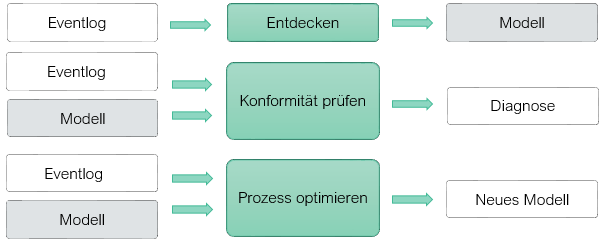
\includegraphics[scale=0.8]{figures/Appbildungen/PM_functions.PNG}
    \caption{Die drei Typen des Process Mining (eigene Darstellung in Anlehnung an: Process Mining Manifest, 2011, S.4, \cite{PMManifesto})}
    \label{fig:pm_functions}
\end{figure}

\newpage
\subsection{Process Mining Typen}
Die drei unterschiedlichen Typen kennzeichenen folgende Eigenschaften und Abläufe:
\begin{itemize}
\item \textbf{Discovery}: Im Ausgangszustand besteht keinerlei a Priori Modell. Der Discovery Vorgang beschäftigt sich damit, den real geschehenden Prozess, anhand der von den verbundenen Geräten hinterlassenen Eventlogs, herauszukristallisieren und ein Prozessmodell aus der gegebenen Historie der Geschehnisse zu erstellen.

\item \textbf{Conformance Checking}: Ein a-priori Modell des Prozesses existiert. \textit{Conformance Checking} vergleicht den real existierenden Ablauf mithilfe des Eventlogs mit dem erwünschten Prozess um festzustellen, ob das beobachtete Verhalten mit dem geplanten Prozess übereinstimmt. Dieser Vorgang ermöglicht die Aufdeckung von Abweichungen zwischen geplanten und tatsächlichen Prozessvorgängen und kann auf Abweichungen hinweisen.  \textit{Conformance Checking} schließt \textit{Compliance Checking} mit ein, d.h. der beobachtete Prozess wird auch daraufhin untersucht, ob er sich an vorgefertigte Regeln, Spezifikationen oder relevante Normen hält.

\item \textbf{Enhancement}: Ein a-priori Modell des Prozesses existiert. Das Ziel ist die Optimierung oder Umgestaltung eines Modells, mithilfe der aus der Auswertung des Eventlogs gewonnenen Informationen. Ein Prozess kann in Bezug auf seine Performanz oder Einhaltung geforderter Standards hin verbessert oder erweitert werden. Informationen wie Kostenanalyse, Zeitaufwand oder Priorisierung einzelner Schritte können in die Optimierung miteinfließen, beobachtete Engpässe können umgangen werden.
\end{itemize}

Aufgabe der Discovery Funktion und Grundlage für alle weiteren Schritte ist die Umwandlung des aufgenommenen Protokolls in ein graphisches Modell; in der Regel handelt es sich dabei um ein Petri Netz. Dies ist eine methodische Darstellungsform, die dazu dient, nebenläufige Prozesse zu beschreiben. Da Petri Netze auch im folgenden praktischen Teil der Arbeit eingesetzt werden, werden sie an dieser Stelle kurz erläutert.

\subsection{Petri Netze}
Formal werden Petri Netze als gerichtete, bipartite Graphen definiert, die aus Stellen  und  Transitionen  bestehen und durch  gerichtete  Kanten  verbunden sind, wie sie in \textit{Software Engineering durch Modellierung wissensintensiver Entwicklungsprozesse} beschrieben sind \cite{freund2007software}. 

Ein Petri-Netz wird formal durch das Tripel $N = (S, T, F)$ definiert. $S$ ist die Menge der Stellen, $T$  ist  die  zu  $S$  disjunkte  Menge  der  Transitionen  und  $F⊆ (S ×  T) ∪ (T  ×  S) $ ist  eine Flussrelation,  welche  die  Menge  der  Kanten  bezeichnet.  Die  Elemente  aus  $S$  werden grafisch repräsentiert durch Kreise, Elemente aus $T$ durch Rechtecke und Elemente aus $F$ als gerichtete Kanten zwischen Stellen und Transitionen. Stellen,  die  sich  vor  Transitionen  befinden, werden Eingangsstellen genannt, Stellen nach Transitionen sind deren Ausgangsstellen. 

\begin{figure}[!h]
    \centering
    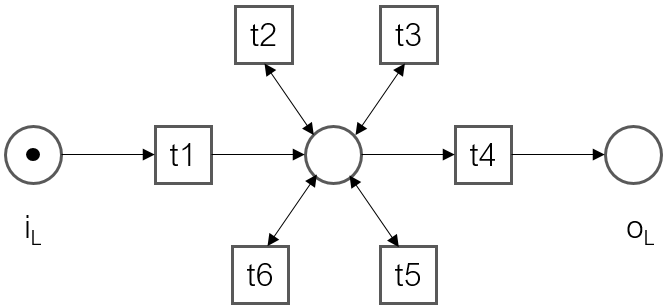
\includegraphics[width=0.65\textwidth]{figures/Appbildungen/petriNetFlower.png}
    \caption{Ein markiertes Petri Netz mit Eingangsstelle $i_L$ und Ausgangsstelle $o_L$}.
    \label{fig:exampleFlower}
\end{figure}

$T$ ist eine endliche Menge von Übergängen für die gilt: $S ∩ T =  ∅.$

$F ⊆(S × T) ∪ (T × S)$ beschreibt eine zweistellige Relation.

Eine  Stelle  $s∈S$  ist  Eingabestelle  einer  Transition  $t∈T$,  wenn  eine  gerichtete  Kante  von $s$ nach $t$ existiert. Eine Stelle $s$ ist Ausgabestelle einer Transition $ t$, wenn eine gerichtete Kante von $t$ nach $s$ existiert. Die Menge aller Eingabestellen einer Transition t wird mit $\cdot t$ bezeichnet und Vorbereich genannt. Die Menge aller Ausgabestellen einer Transition $t$ wird mit $t \cdot$ bezeichnet und Nachbereich genannt. Ein Beispiel für ein Petri Netz bestehend aus drei Stellen und sechs Transition ist in Abbildung \ref{fig:exampleFlower} zu sehen.

Markierungen definieren die Semantik der Netze. Jede Stelle kann eine oder mehr Markierungen beinhalten, die illustriert als Punkt auf der jeweiligen Stelle markiert werden. Eine Transition kann aktiv werden, wenn auf jeder Stelle, von der aus eine Kante zu dieser Transition führt, mindestens eine solche Markierung liegt. Eine aktive Transition kann schalten, indem sie von allen Eingangsstellen eine Markierung entfernt und zu jeder Ausgangsstelle eine Markierung hinzufügt. Damit sind Transitionen aktive Einheiten und ermöglichen so die Darstellung der legitimen Aktivitäten eines Prozesses, vgl. \cite{Petrinetze}.
\newpage
\subsection{Qualitätskriterien}\label{sec:quality}
Für die Bewertung der Qualität eines Ausgabemodels  bedarf es fester Kriterien. Diese unterscheiden sich jedoch je nach Anwendungsfall gravierend in ihrer Bedeutung, da die Ansprüche an ein Ausgabemodell abhängig von der beabsichtigen Verwendung des Modells und der Zielgruppe sind, die das Modell zielführend interpretieren soll. In der Literatur werden meist folgende vier Dimensionen zur Beurteilung herangezogen \cite{PMinAction}:

\begin{itemize}
\item \textbf{Fitness}: Eine perfekte Fitness bedeutet, dass das Prozessmodell das Verhalten aus dem Eventlog vollständig wiedergibt. Sie beschreibt den Grad zu dem Prozesse in der Realität durch das Modell abgedeckt werden.
 
\item \textbf{Precision}: ein Maß, das beschreibt, ob das Modell Verhalten erlaubt, das grundlegend verschieden von dem im Eventlog aufgezeichneten ist. Ein Modell mit geringer Präzision ist \textit{unterformt}, das heißt, es lässt sowohl Verhalten zu, das sich aus dem Eventlog ergibt als auch viele weitere Ereignisketten. Dadurch ist die Aussagekraft des Modells niedrig. Es entsteht dabei ein sogenanntes Blumenmodell, bei dem von einer Transition aus viele Stellen beliebig oft erreichbar sind, entsprechend Abbildung \ref{fig:exampleFlower}.

\item \textbf{Generalization}: Die Generalisierung gibt an, in wie weit das Verhalten aus dem Eventlog im Ausgabemodell verallgemeinert wurde. Ein Modell soll generalisieren, dabei aber nicht das Verhalten welches in dem Eventlog vorhanden ist einschränken. Man sagt ein \textit{überformtes} Modell generalisiert nicht genug - Abläufe die Teil des Modells sein sollten, werden nicht repräsentiert.

\item \textbf{Simplicity}: Die Komplexität des Ausgabemodells sollte auf ein Minimum reduziert werden. Dies steht in einem engen Konflikt mit den anderen zuvor genannten Dimensionen. Ihr Maß sollte gemeinhin der Zielgruppe und dem Anwendungsfall angepasst werden. Ein Modell, das die Wirklichkeit akkurat wieder gibt, aber vom Anwender nicht interpretiert werden kann, erfüllt seinen Zweck nicht. Wird das Modell wiederum zu stark vereinfacht, können für den Anwender relevante Informationen ausgeblendet werden.
\end{itemize}

Da diese Dimensionen in einer Wechselbeziehung zueinander stehen und sich gegenseitig beeinflussen, ist es je nach Kontext notwendig sie gegeneinander abzuwägen. In vielen Fällen soll das Ausgabemodell ein möglichst detailgetreues Abbild des Verhaltens aus dem Eventlog nachbilden, also auch die Mehrzahl der auftretenden Muster wiedergeben. 
Es kann je nach Anwendungsfall aber wünschenswert sein, eine möglichst einfache und wenig komplexe Abstraktion aus dem Eventlog zu generieren, welches dann bewusst auf selten auftretende Muster verzichtet und aus einer möglichst geringen Anzahl aus Stellen und Transitionen besteht. Dieser Faktor sollte vom Anwender des Process Mining berücksichtigt werden, bevor die Prozessanalyse beginnt.

\subsection{Herausforderungen}\label{challanges}
Process Mining kann nur dann aufschlussreiche Antworten auf Fragen nach Prozesstrukturen liefern, wenn die Daten, mit denen es arbeitet, vordefinierte Kriterien erfüllen. Wie in anderen Gebieten der Datenanalyse gilt auch hier das Prinzip \textit{Garbage in, Garbage out} \cite{GIGO}. 

\subsubsection{Rauschen}
Eine der größten Fehlerquellen des Process Mining ist Rauschen in den zur Verfügung stehenden Daten. Um ein Modell zu erzeugen, das möglichst wenig von dem reellen Prozess abweicht, muss angenommen werden, dass das Eventlog, das als Input dient, alle tatsächlich auftretende Vorgänge vollständig widerspiegelt. Wenn viele Einträge, relativ zur insgesamt erfassten Datenmenge gemessen, im Eventlog vorliegen, die irrelevant sind oder als Ausnahmesituation gewertet werden, wird der Process Mining Algorithmus nicht oder nur schlecht in der Lage sein, diese als Rauschen zu identifizieren. Es ist dann wahrscheinlich, dass fehlerbehaftete Muster erkannt werden, die dem realen Prozess nur teilweise entsprechen oder in gravierenden Fällen diesem vollkständig widersprechen.

Ein Ansatz, um den Einfluss von Rauschdaten zu reduzieren ist es, systematisch Schwellwerte für ihre Auftrittshäufigkeit zu finden, so dass Rauschdatensätze herausgefiltert werden, bevor die eigentliche Analyse einsetzt. 

\subsubsection{Unvollständigkeit}
Sind zu wenige Daten vorhanden oder werden umfangreiche Prozesse nicht detailgetreu dokumentiert, kann Process Mining nicht garantieren, dass das resultierende Modell vollständig ist. 
Fehlende Informationen können manuell in der Vorverarbeitung der Daten nachgetragen werden, verlangsamen aber den Analyseprozess und sind fehleranfälliger als automatisiertes Sammeln und Eintragen von Informationen. 

Nicht nur Mangel an korrekt deklarierten Attributen, auch im Protokoll nicht dokumentierte Ereignisse, die aber im realen Ablauf essentiell für den Prozess sind, können dazu führen, dass ein Modell unvollständig ist. Eine weitere Fehlerquelle ist der umgekehrte Fall, wenn Einträge aufgezeichnet wurden, obwohl bestimmte Aktivitäten nicht stattgefunden haben, beispielsweise im Vorfeld eingetragene Termine die nachträglich abgesagt wurden, ohne dass dies im System vermerkt wurde. 

Ein Prozesschritt kann auch unerkannt bleiben, obwohl er im Eventlog dokumentiert wird. Dies kann geschehen wenn die Dokumentation zu kleinschrittig bleibt, als dass erkannt werden kann, um welchen übergreifenden Prozesschritt es sich handelt. 

Um das Problem der Unvollständigkeit zu vermeiden, muss vor der Analyse sichergestellt werden, dass jede für den Prozess relevante Instanz automatisch Einträge im Eventlog generiert, sobald neue Aktionen eintreten. Außerdem muss  verhindert werden dass Einträge entstehen, die nicht der Realität entsprechen.

\subsubsection{Parallele Abläufe}
Die Einträge eines Eventlogs liegen stets in sequentieller Form vor, was das Aufdecken von parallel ablaufenden Vorgängen erschwert. Falls Anfang und Ende der Aktivitäten protokolliert werden, erleichtert dies die korrekte Modellierung. In den meisten Systemen werden Aktivitäten jedoch als atomare Vorkommnisse im Eventlog vermerkt. Dann muss in der Analyse, aus dem verschachtelten Auftreten von Prozessen in einer Vielzahl von Einträgen, auf die Parallelität geschlossen werden. Liegen nur wenige Einträge vor, sinkt auch die Wahrscheinlichkeit, dass parallele Abläufe korrekt klassifiziert werden. Die Strategie, mit der parallele Sequenzen von Process Mining Algorithmen erkannt werden, kann sich von Verfahren zu Verfahren stark unterscheiden und unterschiedlich zuverlässig ausfallen.

\subsubsection{Schleifen}
Ein weiteres Hindernis für Process Mining Algorithmen ist die korrekte Identifizierung von zyklischen Abläufen in einem Eventlog. Insbesonders kurze Schleifen, bestehend aus nur einer oder zwei Aktivitäten, sind für einfache Process Mining Verfahren schwierig zu erkennen. 
Wenn der Protokollierungsmechanismus um die Funktion erweitert wird, zyklische Abläufe zu nummerieren, kann die korrekte Modellierung erleichtert werden. Diese Funktion kann aber nicht in jedem System als gegeben vorausgesetzt werden.

%Im Gegensatz zu Rauschdaten, die durch einen Fehlerhaften  Protokollierungsvorgang hervorgerufen werden, können Ausnahmefälle und fehlerhafte Instanzen für eine Evaluation des Prozesses von größerem Interesse sein, wenn der Andwendungsfall vorsieht Abweichungen zu einem organisierten Prozess zu entdecken. 

%Sie können für den Modellierungsprozess aber irrelevant sein, wenn das Ziel ist ein möglichst generisches Modell zu erzeugen, dann müssen die Ausreißer im Protokoll durch ausreichend korrekte Abläufe anteilsgemäß aufgehoben werden. 

%Der erfolgreiche Einsatz von Process Mining Algorithmen setzt außerdem voraus, dass der Prozess vom EreignisEventlog bis hin zur Interpretation des Modells begleitet wird von Personen, die sowohl mit den Stärken und Schwächen der Process Mining Methode vertraut sind, als auch den Eigenschaften der untersuchten Umgebung sowie den Einsatzzweck des Process Mining kennen und darüber hinaus wissen, wie gegebene Parameter des eingesetzten Verfahrens anzupassen sind, wie die Eingangsdaten aufbereitet werden müssen und wie weit die Aussagekraft des Ergebnismodells reicht. (entfernen?)
\section{Process Mining Algorithmen}
Die Grundlage für die allermeisten algorithmischen Verfahren zur Konstruktion von Prozessmodellen sind Ordnungsrelationen. Im Process Mining beschreiben sie die Beziehung, oder das fehlen einer Beziehung, zwischen zwei Elementen eines Prozesses. 

Als ein verbreitetes  Beispiel für ein rein algorithmisches Verfahren zur Prozessentdeckung, das auf Ordnungsrelationen basiert, kann der $\alpha$-Algorithmus genannt werden, dessen Ablauf unter \textbf{ Algorithmus \ref{alg:alphaminer}} einsehbar ist.
Es handelt sich dabei um eine sehr einfache Variante eines Process Mining Algorithmus, der für wenig komplexe Eventlogs aber, nach den zuvor beschriebenen Qualitätskriterien, korrekte Modelle erstellen kann. Er soll hier als einleitendes Beispiel für Process Mining \textit{Discovery} im Allgemeinen näher betrachtet werden. \newline

\providecommand\algorithmname{alphaminer}
\begin{algorithm}
  \caption{Alpha Miner}
  \label{alg:alphaminer}
  \begin{algorithmic}[1]
    \State $T_L = \{ t \in T \;\mid \exists_{\sigma \in L} \; t \in \sigma\}$ \label{op0}
    
    \State $T_I = \{ t \in T \;\mid \exists_{\sigma \in L} \; t=first(\sigma)\}$ \label{op1}
    
    \State $T_O = \{ t \in T \;\mid \exists_{\sigma \in L} \; t=last(\sigma)\}$ \label{op2}
    
    \State $X_L = \{ (A,B) \mid A \subseteq T_L \land A \neq $\o$ \land B \subseteq T_L \land B \neq $\o$ \land \forall_{a\in A} \forall_{b\in B}\; a \to _L b \land \forall_{a1,a2\in A} a_1 \# _L a_2 \land \forall_{b1,b2\in B} b_1 \# _L b_2\}$ \label{op3}
    
    \State $Y_L = \{ (A,B) \in X_L \mid \forall_{A',B' \in X_L} A \subseteq A' \land B \subseteq B' \implies (A,B) = (A',B')\}$ \label{op4}
    
    \State $P_L = \{ p_{(A,B)} \mid (A,B) \in Y_L \} \cup \{i_l, o_L \}$ \label{op5}
    
    \State $F_L = \{ (a,p_{(A,B)}) \mid (A,B) \in Y_L \land a \in A \} \cup \{  (p_ {(A,B)},b) \mid (A,B) \in Y_L \land b \in B \} \cup \{ (i_l,t \mid t \in T_I  \} \cup \{ (t,o_L \mid t\in T_o\}$ \label{op6}
    
    \State $\alpha(L) = (P_L, T_L, F_L) $ \label{op7}
    
  \end{algorithmic}
\end{algorithm}

Das Verfahren arbeitet mit verlaufsdatenbasierten Ordnungskriterien (\textit{Eventlog-based ordering relations}). Auf die kausale Beziehung zwischen Aktivitäten $(a→b)$ wird geschlossen, wenn zwei Aktivitäten $a$ und $b$ mindestens einmal in der Sequenz $(ab)$ im Eventlog vorkommen, und die Sequenz $(ba)$ nie auftritt. Auf parallele Ausführung zweier Aktivitäten $(a|b)$ wird durch die Verschränkung dieser Aktivitäten geschlossen. Auf die Unabhängigkeit zweier Aktivitäten $a$ und $b$ $(a\#b)$ wird geschlossen, wenn weder die Sequenz $(ab)$ noch die Sequenz $(ba)$ im Eventlog vorkommt.

Im ersten Schritt des Verfahrens werden alle Aktivitäten des Eventlogs in einer Menge zusammengefasst. In Schritt 2 und 3 des Algorithmus werden die Mengen der ersten und letzten Elemente aller Sequenzen in einer Menge gesammelt. 
Schritte 4 und 5 stellen den eigentlichen Kern des $\alpha$-Miner Algorithmus dar. Die Positionen und die Verbindungen der Elemente müssen systematisch ermittelt werden. Es sollen Knoten $p(A,B)$ der Art entstehen, dass $A$ die Menge der Übergangseingänge ist und $B$ die Menge der Übergangsausgänge. Alle Elemente der Menge $A$ sollen in einer kausalen Beziehung zu den Elementen der Menge $B$ stehen, die Elemente der Menge stehen dabei nicht in einer Beziehung zu Elementen der eigenen Menge.

In Schritt 6 werden außerdem die Knoten $i_L$ und $o_L$ festgelegt, dabei handelt es sich um die Anfangs- und Endknoten des zu konstruierenden Netzes, sie werden auch als \textit{Source} beziehungsweise \textit{Sink} bezeichnet. Schritt 7 des Algorithmus ist verantwortlich für die Erzeugung der Kanten des Netzes, entsprechend der Beziehung zwischen den Knoten, die durch eine Kante verbunden werden. Abschließend wird in Schritt 8 das gesamte Netz aus den zuvor bestimmten Netzkomponenten zusammengesetzt und der Algorithmus endet.
\newpage
\subsection{Beispiel einer Analyse einer Protokolldatei}
Das Ausgabemodell einer Process Mining Discovery Analyse über der selben Protokolldatei kann, in Abhängigkeit von der Strategie des eingesetzten Process Mining Verfahrens, variieren. Process Mining Algorithmen ähneln sich jedoch größtenteils in ihrer grundlegenden Struktur. Um den im vorangegangen Abschnitt vorgestellten Algorithmus verständlich zu machen, soll hier exemplarisch eine Auswertung durch den $\alpha$-Miner Algorithmus schrittweise nachvollzogen werden.

Da der Schwerpunkt dieser Arbeit auf dem Entdecken von Prozessen, also dem Process Mining Typ \textit{ Discovery} liegt, werden im Rahmen dieser Arbeit Process Mining Verfahren betrachtet, die auf der Definition des \textit{General Process Discovery Problem} (Problem der allgemeinen Prozessentdeckung) beruhen. Der folgende Definition stammt aus 'Process Mining in Action' von Wil van der Aalst, 2016, S.163 \cite{PMinAction}:
\begin{addmargin}[20pt]{20pt} 
Man betrachte ein Eventlog $L$ und eine Menge $A$ an Aktivitäten. Eine einfache Sequenz $\sigma$ sei eine Folge von Aktivitäten, sprich $\sigma ∈ A $. Ein Eventlog $L$ setzt sich zusammen aus mehreren Sequenzen über $A$, also ist $L ∈ B(A)$. Ein Process Discovery Algorithmus ist eine Funktion $\gamma$ die einen Input $L$ auf ein Prozess Modell derart abbildet, das es das aufgenommene Verhalten repräsentiert.
\end{addmargin}
Eine gute Repräsentanz ist dann gefunden, wenn die vier Qualitäten des Ausgabemodells (\textit{Fitness, Precision, Generalization, Simplicity}) ein für den Anwendungsfall akzeptables Gleichgewicht erreichen \cite{PMinAction}.

Man betrachte ein Eventlog der Form: $L = [(a, c, d)^6, (b, c, d)^5, (a, c, e)^4, (b, c, e)^2]$.
Die Ordnungsrelation der Elemente des Eventlogs $L$ ist in Tabelle \ref{tab:Ordnungsrelation} aufgeführt.
\begin{table}[!ht]
\centering
\resizebox{\columnwidth/3}{!}{%
\begin{tabular}{cccccc}
 & \textbf{a} & \textbf{b} & \textbf{c} & \textbf{d} & \textbf{e} \\ \cline{2-6} 
\multicolumn{1}{c|}{\textbf{a}} & \multicolumn{1}{c|}{\textit{\#}} & \multicolumn{1}{c|}{\textit{\#}} & \multicolumn{1}{c|}{→} & \multicolumn{1}{c|}{\textit{\#}} & \multicolumn{1}{c|}{\textit{\#}} \\ \cline{2-6} 
\multicolumn{1}{c|}{\textbf{b}} & \multicolumn{1}{c|}{\textit{\#}} & \multicolumn{1}{c|}{\textit{\#}} & \multicolumn{1}{c|}{→} & \multicolumn{1}{c|}{\textit{\#}} & \multicolumn{1}{c|}{\textit{\#}} \\ \cline{2-6} 
\multicolumn{1}{c|}{\textbf{c}} & \multicolumn{1}{c|}{\textit{←}} & \multicolumn{1}{c|}{\textit{←}} & \multicolumn{1}{c|}{\#} & \multicolumn{1}{c|}{\textit{→}} & \multicolumn{1}{c|}{\textit{→}} \\ \cline{2-6} 
\multicolumn{1}{c|}{\textbf{d}} & \multicolumn{1}{c|}{\textit{\#}} & \multicolumn{1}{c|}{\textit{\#}} & \multicolumn{1}{c|}{←} & \multicolumn{1}{c|}{\textit{\#}} & \multicolumn{1}{c|}{\textit{\#}} \\ \cline{2-6} 
\multicolumn{1}{c|}{\textbf{e}} & \multicolumn{1}{c|}{\textit{\#}} & \multicolumn{1}{c|}{\textit{\#}} & \multicolumn{1}{c|}{←} & \multicolumn{1}{c|}{\textit{\#}} & \multicolumn{1}{c|}{\textit{\#}} \\ \cline{2-6} 
\end{tabular}%
}
\caption{Ordnungsrelation zu einem Eventlog $L$ auf Basis des $\alpha$-Miner Verfahrens}
\label{tab:Ordnungsrelation}
\end{table}
\newline
Da auf Aktivität $a$ $c$ folgt, aber auf $c$ nie $a$ folgt, besteht die kausale Beziehung $(a→c)$ und man erwartet, dass ein Modell zu dem Eventlog diese Beziehung reflektiert.

Die Relationsmatrix aus Tabelle \ref{tab:Ordnungsrelation} lässt sich auch als eine Menge aus Tupeln wie folgt darstellen:

$ X_L={ [({a}, {c}), ({b}, {c}), ({c}, {d}), ({a}, {c, e}),
({a}, {c, d}), ({b}, {d}), ({c}, {d}), ({a}, {d}),
({b, c}, {d}), ({b, c}, {e}) ]}$

Wenn ein Knoten für jedes Element der Menge entstünde, würde die Anforderung der Generalisierung verletzt werden. Aus diesem Grund wird eine Bedingung „Maximales Pair“ $(A,B)$ definiert und die Elementmenge gefiltert. Konkret werden alle redundanten Elemente der Menge der Länge zwei entfernt. Es entsteht:

$ X_L={ [({a}, {c, e}), ({a}, {c, d}),
({b, c}, {d}), ({b, c}, {e}) ]}$

Nach Ausführung aller Schritte des $\alpha$-Miners auf das Eventlog $L$ entsteht folgendes Petri Netz:

\begin{figure}[!h]
    \centering
    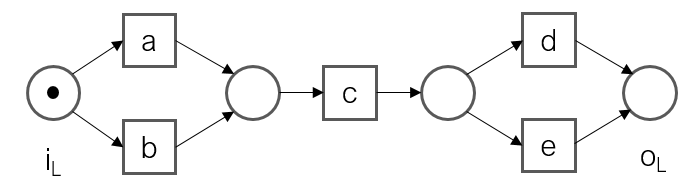
\includegraphics[scale=0.6]{figures/Appbildungen/alpha_petri_net.png}
    \caption{Petri Netz, Resultat des Alpha Miner Verfahrens (eigene Darstellung in Anlehnung an: Aalst, Process Mining, 2016, S.170, \cite{PMManifesto})}
    \label{fig:petriNetExample}
\end{figure}

Der $\alpha$-Miner Algorithmus ist aufgrund seines simplen Aufbaus nicht in der Lage, jede Prozessfolge korrekt zu identifizieren und zu modellieren, beispielsweise werden parallele Abläufe und kurze Schleifen nur unzureichend erkannt.

Um die Probleme in der Prozessanalyse zu bewältigen und Process Mining verschiedenen Anforderungen gegenüber anzupassen, sind im Laufe der Jahre eine Reihe an fortgeschrittenen Algorithmen entwickelt worden, die für unterschiedliche Anwendungsfälle jeweils eigene Vor- oder Nachteile mitbringen können. 

Ein Beispiel für einen Algorithmus, der auf Basis des Alpha Miner entwickelt wurde, ist der Heuristic Process Miner.

\subsection{Heuristic Process Miner}
Der Heuristic Miner basiert auf den Grundlagen des $\alpha$-Miner, arbeitet aber mit zusätzliche Kriterien, die beim Erzeugen des Modells berücksichtigt werden. Wie der Name des Verfahrens vermuten lässt, nutzt der Miner eine Heuristik um zu bewerten, welche Abfolgen tatsächlich Teil des resultierenden Modells werden sollten, konkret wird hierfür die Häufigkeit von Nachfolgerelationen berücksichtigt, vgl.\cite{heurMining}.

Das Verfahren unterscheidet sich kaum von der Vorgehensweise des $\alpha$-Miners, allerdings wird statt lediglich zu unterscheiden, ob eine direkte Folge zwischen zwei Knoten besteht oder nicht, eine Beziehung zwischen zwei Elementen $a$ und $b$ über einen numerischen Wert gewichtet. Das Gewicht der Kante entspricht der Relevanz der Folgebeziehung im Modell. Es wird berechnet über die Formel: 
\begin{equation}
 {a} \Rightarrow _L {b} = \left(\frac{ | {a} >_L {b} - {b} >_L {a} }{|{a} >_L {b}| + |{b} >_L {a}| + 1 }\right)
 \end{equation}
 Dabei beschreibt $|{a} >_L {b}|$ die Häufigkeitsmenge, mit der $b$ auf $a$ in $L$ folgt, wobei $L$ das Eventlog über der Menge der Protokolleinträge darstellt. Die berechneten Werte liegen zwischen 1 und -1, Werte um den Bereich Null deuten auf darauf hin, dass zwei Einträge unabhängig sind, positive Werte nahe 1 deuten auf eine Abhängigkeitsbeziehung hin, negative auf eine Abhängigkeitsbeziehung in umgekehrter Richtung, also gilt:
 \begin{equation}
 {a} \Rightarrow _L {b} =  -1 \cdot ( {b} \Rightarrow _L{a} )
 \end{equation}
Schleifen der Länge eins stellen bis hier hin weiterhin ein Problem für das Verfahren dar, da die Kante von einem Knoten a zu sich selbst mit niedrigen Werten gewichtet wird. Um dies zu umgehen wird eine Abwandlung der Formel (1) für kurze Schleifen eingeführt:
 \begin{equation}
 {a} \Rightarrow _L {a} = \left(\frac{ | {a} >_L {a}}{
|{a} >_L {a}| + 1 }\right)
 \end{equation}
Anhand dieser Formel kann eine Relationstabelle, entsprechend der Tabelle \ref{tab:Ordnungsrelation} in der Einführung, angelegt werden. Der Heuristics Miner nutzt aber statt der symbolischen Werte, die zwischen vier Zuständen unterscheiden, nun das Gewicht der zugehörigen Kanten. 

Als nächstes berechnet das Verfahren drei Schwellwerte, die jeweils dazu dienen, Rauschen von relevanten Daten zu unterscheiden. Der Schwellwert dient dazu zu entscheiden, ob es sich bei einem Eintrag um Ausreißer in der Datenmenge, oder aber um sporadische, aber für das Modell entscheidende, Ereignisse handelt. Abschließend wird basierend auf den berechneten Abhängigkeitswerten ein Modell generiert.

Der Heuristics Miner kann im Gegensatz zum $\alpha$-Miner auch kurze und lange Schleifen korrekt wiedergeben, muss aber mit zusätzlichen Metriken arbeiten um sogenannte\textit{ long distance dependencies}, also Abhängigkeiten in großer zeitlicher Distanz, zu erkennen.

\subsection{Inductive Process Miner}\label{sec:inducMiner}
Der Inductive Miner ist nach dem Heuristic Miner entwickelt worden und verfolgt die Strategie des \textit{divide and conquer}, um ein Modell aus einem gegebenen Eventlog zu erzeugen, vgl. \cite{inducMining}. 
Die Strategie des Inductive Miners ist es, jedes Eventlog $L$ rekursiv in Sub-Eventlogs $A_1 , ... , A_n$ zu unterteilen, diese isoliert zu betrachten und dann in weitere Sub-Eventlogs zu teilen. 
Ziel der Betrachtung eines Sub-Eventlogs ist es zu erkennen, an welcher Stelle des Modells ein sogenannter \textit{Cut} notwendig ist, der definiert, an welcher Stelle das betrachtete Eventlog in Sub-Eventlogs unterteilt wird. An die Stelle des Cuts setzt der Algorithmus eine von mehreren Übergängen. Die Menge an Übergangsmöglichkeiten im Prozess zwischen einzelnen Knoten ist dabei konkret $Oder$, $exklusives  Oder$, $Und$ sowie $Sequenzen$ und $Schleifen$. 

\newpage
Gibt es einen Pfad von $A_i$ nach $A_j$, so dass gilt $ i < j $, besteht eine Sequenz der Form $ → (A_1 , ... , A_n)$ in dem betrachteten Sub-Eventlog.
Besteht beispielsweise keine Abhängigkeit zwischen betrachteten Sub-Eventlogs wird ein Exklusiv Oder als Cut zwischen den Teilelementen, also $ × (A_1 , ... , A_n)$ gesetzt. 
Hat jedes betrachtete Sub-Eventlog einen erkennbaren Anfangs- und Endknoten und sind seine Elemente in einer eindeutigen Sequenz angeordnet, deutet dies auf einen parallelen Übergang $ ∧ (A_1 , ... , A_n)$ hin. 

Dieser rekursive Vorgang wird fortgesetzt bis das betrachtete Sub-Eventlog atomar ist. Ein solcher Cut, bei dem eines der resultierenden Eventlogs atomar ist, ist in Abbildung \ref{fig:imExample} zu sehen. Im letzten Schritt des Inductive Miner Verfahrens werden alle Elemente und ihre Übergänge zu einem einzigen kohärenten Modell zusammengesetzt, vgl. \cite{inducMining}. Das Inductive Mining Verfahren zeichnet sich dadurch aus, dass es sich besonders für den Umgang mit großen Datensätzen und selten auftretenden Ereignissen eignet, vgl. \cite{minerEval}.

\begin{figure}[!h]
    \centering
    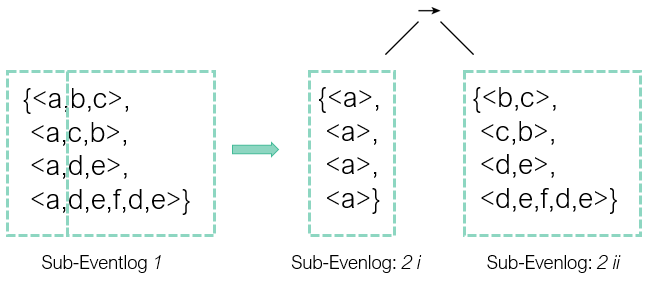
\includegraphics[scale=0.5]{figures/Appbildungen/im_example.PNG}
    \caption{Beispiel einer Trennung eines Eventlogs nach dem Inductive Miner Verfahren}
    \label{fig:imExample}
\end{figure}

Mehrere Varianten des Inductive Miners wurden entwickelt, die das hier vorgestellte Verfahren erweitern, um bestimmte Schwächen des Verfahrens zu umgehen oder den Algorithmus für spezifische Anwendungsfälle anzupassen. 
Beispielsweise kann das Protokoll selten auftretendes, aber für den Kontext relevantes Verhalten enthalten, was Algorithmen zwingt, diese Einträge entweder auszuschließen oder komplizierte, unlesbare Modelle auszugeben, die jeden beliebigen Prozess beschreiben, also einem  Blumenmodell wie in Abbildung \ref{fig:exampleFlower} entsprechen. Um dieses Problem schnell und effektiv zu lösen ist der Inductive Miner \textit{infrequent}, kurz IMf entwickelt worden, vgl.  \cite{inducFMining}.

Ein anderes häufig auftretendes Problem, ist ein Protokoll das unzureichende Informationen enthält, um ein Prozessmodell zu finden, das die Realiät korrekt abstrahiert. Unvollständigkeit zwingt Algorithmen, entweder das fehlende Verhalten auszuschließen und damit das noch unsichtbare Verhalten zu reduzieren, das das Modell erzeugen kann, oder das fehlende, unbekannte Verhalten dort einzubeziehen, indem sie das Risiko eingehen, falsch zu raten. Im Hinblick auf diese Problematik ist der Inductive Miner \textit{incomplete}, kurz IMc entstanden, vgl. \cite{inducIMining}.

\subsection{Local Process Miner}
Der Local Process Miner ist eines der jüngsten Verfahren der Discovery Process Miner. Im Jahr 2016 im 'Journal of Innovation in Digital Ecosystems' vorgestellt \cite{localMining}, basiert es auf den Erkenntnissen aus der Entwicklung des Sequential Pattern Mining \cite{Srikant1996MiningSP} und des Episode Mining \cite{mannila1997discovery}.

Der Local Process Miner unterscheidet sich von den anderen, hier vorgestellten Algorithmen, dadurch, dass er nicht ein, sondern mehrere Modelle erzeugt. Die Modelle beschreiben dabei häufiges, aber partielles Verhalten und bestehen  aus nicht mehr als drei bis fünf Einträgen. Das heißt jedes einzelne der entstandenen Netze modelliert nur eine Teilmenge der Aktivitäten, die in der Protokolldatei beobachtet werden. Der Algorithmus lässt sich in vier iterativen Schritten zusammenfassen: der initialen Generation, der Evaluation, der Selektion und der Expansion. LPM baut auf sogenannten Process Trees auf, der Prozess wird also als Baumstruktur beschrieben. Die  Kindknoten des Baumes werden als Nachfolger von Elternknoten abstrahiert. Die Knoten repräsentieren, wie beim Petri Netz auch, einzelne Ereignisse beziehungsweise Einträge eines Eventlogs oder Übergänge zwischen den Einträgen. 

Zunächst wird eine Menge von einblättrigen Prozessbäumen $CM_1$, $i=1$ generiert. Jedes Blatt entspricht einem Eintrag des zu analysierenden Eventlogs. Die gegebene Menge wird nach vordefinierten Qualitätskriterien evaluiert. Auf Basis der Evaluation wird eine Teilmenge $SCM_i \subseteq CM_i$ ausgewählt. In diesem Schritt prüft die Abbruchbedingung, ob die nutzerdefinierte maximale Anzahl an Iterationsschritten erreicht wurde oder die Teilmenge $SCM_i=∅$  ist. Wird eine der beiden Bedingungen erfüllt, endet der Algorithmus. Werden sie nicht erfüllt, folgt Schritt vier, die Expansion. 

In jedem Expansionsschritt wird die Menge aus einzelnen Prozessbäumen zu einer Menge aus größeren Bäumen $CM_i+1$ erweitert. Bei der Expansion wird jeder Knoten ersetzt durch einen Sub-Prozessbaum, der diesen Knoten enthält. Beispielsweise ist eine mögliche Erweiterung von $a$: $ →(a,b)$, die als neues Element der Menge $CM_2$ deklariert wird, wie in Abbildung \ref{fig:lpmExample} zu sehen ist. 
\begin{figure}[!h]
    \centering
    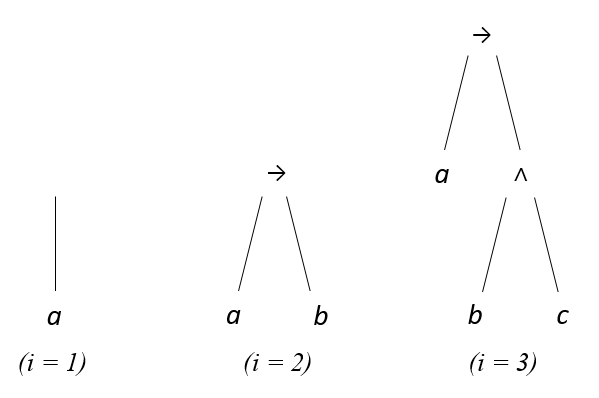
\includegraphics[scale=0.4]{figures/Appbildungen/lpm_example.PNG}
    \caption{Ein initialer Prozessbaum und seine Expansion im Local Process Miner, (eigene Darstellung in Anlehnung an: Dalmas B., N. Tax, 2017, S.5, \cite{lpm}) }
    \label{fig:lpmExample}
\end{figure}

An den Expansionsschritt knüpft wieder ein Selektionsschritt an, die Selektion erfolgt über eine Reihe von für den gegebenen Eventlog berechneten Schwellwerten, vgl. \cite{lpm}. Die resultierenden Prozessbäume können abschließend in Petri Netze überführt werden.

Die für das Local Process Mining charakteristischen kurzen Ausgangsmodelle sind nicht, oder nur unzureichend, geeignet, um dem Anwender einen Eindruck von langkettigen Prozessen zu verschaffen und Prozesse grob zu abstrahieren. Allerdings sind die Ausgangsmodelle besser als andere gängige Process Mining Algorithmen dazu geeignet, Detailansichten von Prozessen zu konstruieren. 
Diese können je nach Anwendungsfall besonders hilfreich sein, um festzustellen welche kleinschrittigen Muster und Routinen sich in einem Prozess verbergen, die von Ausgabemodellen, die einen Prozess vollständig abdecken wollen, häufig übergangen werden. Allerdings ist dieses Verfahren bisher sehr rechenintensiv, was auch darauf zurück zu führen ist, dass seit seiner Veröffentlichung nicht genug Zeit vergangen ist, entsprechend optimiert zu werden, vgl. \cite{localMining}.

%Die Wahl eines Verfahrens sollte entsprechend nicht allein darauf beruhen, evtl. mehr bla bla 

\section{Protokolldateien}
\subsection{Tabellarische Eventlogs}
Nachdem im vorangegangenem Kapitel auf die verschiedenen Prozess Mining Algorithmen eingegangen wurde, sollen in diesem Kapitel die, allen Verfahren gemeinen, Ein- und Ausgangsdaten näher betrachtet werden.
In praktischen Anwendungen liegen die Eingangsdaten in der Regel als Protokolldateien vor. Die Beschaffenheit der in dieser Arbeit verwendeten  Protokolldateien, die als Basis für die die Analyse und letztendliche Erzeugung von Petri Netzen dienen, soll hier wieder anhand eines Beispiels beschrieben werden.

Um einen Prozess basierend auf einer Protokolldatei erkennen zu können, muss die Datei zunächst einem formalen Schema folgen. Es können der Zeitstempel des Eintrags, die Ressource, die den Eintrag einleitet, sowie verschiedene Attribute der jeweiligen Ressource, die den Zustand oder die Lokalisation beschreiben, in der Protokolldatei hinterlegt werden, vgl. \cite{PMinAction}.

Tabelle \ref{tab:example-Eventlog} zeigt ein fiktives Protokoll, welches auch Teil der nachfolgenden Versuchsreihe ist. 
\begin{table}[!ht]
\centering
\resizebox{280pt}{!}{%
\begin{tabular}{l|lll}
\textbf{case} & \textbf{timestamp} & \textbf{resource} & \textbf{activity} \\ \hline \hline
AA & 2019-01-01 07:36:36 & Coffee maker & turned to ON \\
AA & 2019-01-01 07:38:03 & Appliance g & read 0 \\
AA & 2019-01-01 07:42:09 & Doorbell & ringing \\
AA & 2019-01-01 07:45:36 & Coffee maker & Two Esprosso Cups \\
AA & 2019-01-01 07:45:42 & Appliance b & read 90 \\
... & ... & ... & ... \\ \hline
AB & 2019-01-02 07:33:27 & Doorbell & ringing \\
AB & 2019-01-02 07:35:51 & Coffee maker & turned to ON \\
AB & 2019-01-02 07:35:57 & Appliance j & read 90 \\
AB & 2019-01-02 07:36:15 & Appliance h & read 67 \\
AB & 2019-01-02 07:42:27 & Coffee maker & Two Esprosso Cups \\
... & ... & ... & ... \\ \hline
AC & 2019-01-03 07:34:30 & Doorbell & ringing \\
AC & 2019-01-03 07:36:54 & Coffee maker & turned to ON \\
AC & 2019-01-03 07:38:21 & Appliance c & read 45 \\
AC & 2019-01-03 07:39:06 & Appliance g & read 13 \\
AC & 2019-01-03 07:43:30 & Coffee maker & Two Esprosso Cups \\
... & ... & ... & ... \\ \hline
AD & 2019-01-04 07:35:33 & Doorbell & ringing \\
AD & 2019-01-04 07:35:57 & Appliance h & read 90 \\
AD & 2019-01-04 07:37:57 & Coffee maker & turned to ON \\
AD & 2019-01-04 07:41:30 & Appliance f & read 67 \\
AD & 2019-01-04 07:43:30 & Coffee maker & Two Esprosso Cups \\
... & ... & ... & ... \\ \hline
\end{tabular}%
}
\caption{Auszug aus Eventlog der Versuchsreihe A in Kapitel \ref{chap:approach}}
\label{tab:example-Eventlog}
\end{table}
Eine grundlegende Annahme der Process Mining Verfahren ist, dass die Ereignisse einer Protokolldatei alle Teil eines zusammenhängenden Prozesses sind. Weiterhin entspricht jeder Eintrag, oder eine Zeile in der Tabelle, jeweils genau einem atomaren Ereignis. Ereignisse die zu einer Prozessinstanz gehören müssen alle mit dem selben sogenannten \textbf{Case} deklariert werden, ein Case bezeichnet einen isolierten Vorgang innerhalb eines Prozesses und kann aus einem oder mehreren Ereignissen bestehen. In Tabelle \ref{tab:example-Eventlog} entspricht ein Case jeweils dem Zeitraum von einem Kalendertag, Cases können auch danach differenziert werden, welche Person mit einem Prozess assoziiert ist, oder beispielsweise bei Supportanfragen anhand der ID des gemeldeten Vorfalls unterschieden werden.

Es wird außerdem mindestens eine Spalte, genannt \textbf{Activity}, benötigt, welche beschreibt, welche Aktion das Ereignis ausgelöst hat. Activities stehen nie für sich allein,  sondern gehören immer zu einer sogenannten \textbf{Resource}, die für die Erzeugung des Eintrags verantwortlich ist. Beispielsweise werden gemessene Sensorwerte (Activity) immer mit der Bezeichnung des Sensors (Ressource) eingetragen. Aktionen die von Personen durchgeführt wurden können die Person als Ressource identifizieren.

Die sequentielle Abfolge der Einträge ist von entscheidender Bedeutung für die Auswertung der Protokolldatei. Liegen neben der Aktivität zur Ressouce auch Zeitstempel (\textbf{Timestamps}) vor, können diese bei der Auswertung zusätzlich berücksichtigt werden. Auf diese Weise fließt die zeitliche Distanzen als Metrik in die Auswertung mit ein. Fehlen Zeitstempel, so wird angenommen, dass die Distanzen zwischen einzelnen Ereignissen mit dem gleichen Wert gewichtet werden können.
Jede weitere Spalte, die Metainformationen liefert, kann die Ausgabequaltät zusätzlich verbessern. Diese Spalten werden auch als die Attribute des Ereignisses bezeichnet. 
\newpage
\subsection{XES Standard}\label{sec:xes}
Um Ereignisprotokolle einheitlich und herstellerunabhängig mit verschiedenen Werkzeugen verarbeiten zu können, wurde 2004 die Mining eXtensible Markup Language (MXML) definiert. Sie wurde durch das eXtensible Event Stream(XES) Format abgelöst \cite{xesmxml} und ist 2016 von der \textit{IEEE Task Force on Process Mining} als Standard anerkannt worden. 

Ein XES Dokument enthält jeweils eine Protokolldatei mit einer beliebigen Anzahl an Ereignissen, in einer festen Abfolge, und beliebig vielen Attributen, die vom Typ, wie beim zugrundeliegenden XML Standard auch, \textit{String}, \textit{Date}, \textit{Int}, \textit{Float} oder \textit{Boolean} sein können. 
Der Anwender kann Attribute als erforderlich deklarieren, neue Attribute definieren oder auf die vom XES Modell definierten Typen zugreifen. XES  wird von einer weiten Bandbreite an Process Mining Software unterstützt und zählt gemeinhin als favorisiertes Datenformat für die Verarbeitung durch Process Mining Algorithmen.

Wird das Ereignisprotokoll aus Tabelle \ref{tab:example-Eventlog} in ein XES Dokument konvertiert, erhält man eine Dokument folgender Struktur:
\small
\lstset{language=XML}
\begin{lstlisting}[label=lst:xes]
<?xml version="1.0" encoding="UTF-8" ?>
    <!-- XES standard version: 1.0 -->
    <!-- OpenXES library version: 1.0RC7 -->
    <!-- OpenXES is available from http://www.openxes.org/ -->
    <Eventlog xes.version="1.0" xes.features="nested-attributes" openxes.version="1.0RC7">
    	<extension name="Lifecycle" prefix="lifecycle"/>
    	<extension name="Time" prefix="time"/>
    	<extension name="Concept" prefix="concept"/>
    	<classifier name="Event Name" keys="concept:name"/>
    	<string key="concept:name" value="XES Event Eventlog"/>	<trace>
		<string key="concept:name" value="AA"/>
		<event>
			<string key="resource" value="Doorbell"/>
			<string key="lifecycle:transition" value="start"/>
			<string key="concept:name" value="Doorbell ringing"/>
			<date key="time:timestamp" value="2019-01-01T07:32:24.000+02:00"/>
			<int key="Event ID" value="100"/>
		</event>
	
\end{lstlisting}
\normalsize
    \chapter{Stand der Technik, Process Mining im Smart Home}\label{chap:stateoftheart}

Generell beschäftigt sich Process Mining mit der Aufgabe, Modelle von realen Prozessen, im Gegensatz zu solchen die von Betrachtern vermutet oder angenommen werden, mit Hilfe von Ereignisprotokollen zu extrahieren, diese zu vergleichen und zu optimieren.\cite{PMinAction}
Dieser Extraktionsprozess von formalisiertem Prozesswissen aus Eventlogs heraus kann in den  unterschiedlichsten Anwendungsgebieten eingesetzt werden, um neue Erkenntnisse über komplexe Abläufe zu erhalten. 

Während der Einsatz in Smart Living Szenarien bisher nur in Ansätzen erforscht wurde, kommt Process Mining in Unternehmen bereits häufiger zum Einsatz, Vgl.\cite{litreview}.

\section{Process Mining im Kontext der Business Analytics und Business Intelligence}

Die Digitalisierung in der Industrie macht durch die gesteigerte Verbreitung von vernetzten Endgeräten rasante Fortschritte und legt dadurch auch das Fundament für die Auswertung großer Datenmengen, in denen Informationen über Prozessabläufe eingebettet sind, Vgl. \cite{GanscharGerlac}. 

In der IT Architektur zahlreicher Unternehmen trifft man häufig auf dezentrale, verteilte technologische Systeme, in denen die unterschiedlichen technologischen Komponenten isoliert, häufig auch als Service eines Drittanbieters, vorliegen , Vgl.\cite{GanscharGerlac}. Dies hat zur Folge, dass an einem einzelnen Prozess unterschiedliche Module, wie das ERP- (Enterprise Ressource Planing), CRM- (Customer Relationship Management) oder SCM-System (Supply Chain Management), beteiligt sind, welche jeweils ihre eigene Informationen zu einem relevanten Prozessablauf bereitstellen. Process Mining kann an dieser Stelle einen entscheidenden Beitrag dazu leisten, festzustellen, ob die internen Abläufe geplanten Prozessen entsprechen und an welchen Stellen diese sich verbessern ließen, Vgl.\cite{PMinAction}.

Process Mining ist außerdem in der Lage Informationen über einen Prozess zu extrahieren, unabhängig davon ob seine Struktur den Teilnehmern des Prozesses oder seinen Organisatoren bekannt ist. Gegenteilig dazu muss bei der Business Process Analysis oder bei dem Business Activity Monitoring zunächst auf a-priori bekannte Geschäftsprozesse zurückgegriffen werden, um diese anschließend zu analysieren. 

Process Mining umfasst dabei nicht allein die Analyse von Abläufen, sondern auch das Entdecken von Zusammenhängen zwischen einzelnen Komponenten und ihren Aktivitäten. Dadurch erübrigt sich bei korrekter Anwendung von Process Mining zur Arbeitsprozessmodellierung, beispielsweise innerhalb eines Unternehmens, die Durchführung von Befragungen der Mitarbeiter zu ihrem Arbeitsprozess. Dies hat zum Vorteil, dass der Einfluss von subjektiven Sichten auf das resultierende Modell minimiert wird und bei der Analyse vergleichsweise zeit- und ressourcenschonend vorgegangen werden kann.
\begin{figure}[!ht]
    \centering
    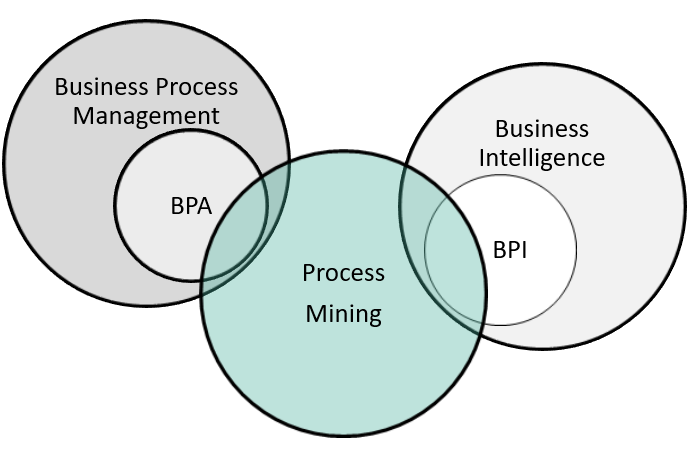
\includegraphics[scale=0.41]{figures/Appbildungen/businessanalytics.PNG}
    \caption{Process Mining im Kontext anderer Verfahren der Unternehmensanalyse,  (Eigene Darstellung in Anlehnung an: Weerdt, J.D., et al., 2013, S.64,\cite{DeWeerdt})}
    \label{fig:BIContext}
\end{figure}

Process Mining kann also als Analysetool, welches sich zwischen der Business Intelligence und dem Business Process Management bewegt, verstanden werden, siehe Abbildung (\ref{fig:BIContext}).

Die Autoren der Metastudie 'Business Process Mining Application: A Literature Review' \cite{litreview} haben aktuelle Veröffentlichungen zum Thema Process Mining auf ihr Anwendungsgebiet hin untersucht und unter anderem herausgefunden, dass in knapp einem Drittel der herangezogenen Literatur Process Mining im Gesundheits- und Pflegedienst eingesetzt worden ist, gefolgt vom IT und Finanzsektor.

\section{Einsatz in der Gesundheits- und Altenpflege}
Eine Studie zum Process Mining in der Geriatrie, die Anfang 2019 im ‚Biomedical Engineering Systems and Technologies Journal‘ erschienen ist \cite{wrro141683}, hat unter allen wissenschaftlichen Veröffentlichungen zum Thema acht Studien identifiziert, die Process Mining erfolgreich in der Altenpflege eingesetzt haben. Bei diesen Studien lag der Fokus nicht allein darauf, einzelne Behandlunsgverläufe und Daten aus den Krankenakten der Patienten systematisch zu analysieren, sondern auch darauf, ihre alltäglichen Handlungensmuster auswerten zu können. 

An dieser Stelle ergibt sich eine Schnittmenge des Process Mining mit dem Forschungsgegenstand der Untersuchung von alltäglichen menschlichen Aktivitäten (englisch \textit{Activities of Daily Living}, kurz ADL). 
Gegenstand einer der einbezogenen Studien war beispielsweise die Pflege von demenzerkrankten Patienten in einem Pfelgeheim, veröffentlicht von Llatas et al. \cite{llatas}, welches mit zahlreichen Sensoren ausgestattet war, deren Eventlogs durch Process Mining ausgewertet wurden. Im Detail wurde hier Conformance Checking eingesetzt. Mithilfe der Auswertung konnten  Differenzen in den Zeitspannen der Alltagsroutinen der untersuchten Patienten beobachtet werden. Eine verlangsamte Routine, oder gravierende Abweichungen zu früheren Tagesabläufen, konnten als frühes Signal einer Veränderung im gesundheitlichen Zustand der Bewohner interpretiert werden.

\section{Process Mining und menschliches Verhalten}
Anhand solcher Studien wird ersichtlich, dass Process Mining auch dem Forschungsfeld der \textit{Human Activity Recognition}, kurz HAR, dienen kann. HAR beschreibt ein Forschungsfeld, das untersucht wie menschliche Aktivitäten, die mit Sensoren aufgenommen wurden, korrekt klassifiziert und auf ihnen zugrundeliegende Muster hin untersucht werden können. 

Events im Eventlog entstehen dann beispielsweise durch Bewegungssensoren, die im Gebäude verteilt werden, Näherungssensoren in elektrischen Geräten und anderen Zustandssensoren, die je zahlreicher und weiter sie gestreut sind, ein klareres Bild über das Verhalten der beobachteten Personen schaffen können. 
Dieser Aspekt unterscheidet Process Mining im Smart Living Kontext vom Process Mining Einsatz im Unternehmen, wo Logs durch meistens durch die bereits vorhandene IT Technik gespeist werden und selten auf die zusätzliche Anreicherung durch Sensoren angewiesen sind.
 
Im Unterschied zur industriellen Umgebung ist die private menschliche Umgebung außerdem gravierenden Schwankungen unterworfen. Dies ist vor allen Dingen dem Umstand geschuldet, dass Unternehmen intern zunächst Arbeitsprozesse planen, definieren und anschließend umsetzen und dabei darauf fokussiert sind, wenig Spielraum für unerwartete Abweichungen im Arbeitsablauf zuzulassen. 
Wie eine Person privat vernetzte Geräte nutzt ist keinem formalen Regelwerk unterworfen. Ein sogenanntes Smart Home ist deutlich weniger reglementiert als eine Fabrik und jeder Anwender entscheidet individuell darüber, welche IoT Geräte wann Teil seines Smart Home werden. Auf diese Weise entsteht in jedem Eigenheim ein individuelles Geflecht aus vernetzten Sensoren und Aktoren, die meist von unterschiedlichen Herstellern stammen, welche selten alle ein und den selben Standards folgen.

Unternehmensinterne Logs sind aus diesem Grund von Beginn an aussagekräftiger als private. Jeder Eintrag lässt sofort Rückschlüsse über die Semantik und den Kontext des Eintrags zu und ist, auch vom Rest des Logs isoliert, interpretierbar. Währenddessen sind Logs aus privaten Umgebungen auf Metainformationen angewiesen, bevor sie interpretiert werden können und einzelne Einträge eines Logs sind, aus dem Kontext der anderen Geräte in ihrer Umgebung herausgenommen, nicht aussagekräftig Vgl.\cite{Jaroucheh2011}.

Ein entscheidender Vorteil der Auswertung von Eventlogs im Smart Home im Hinblick auf Privatsphäre und Datenschutz jedoch ist, dass sie von den beobachteten Personen eher akzeptiert wird als eine Überwachung durch beispielsweise Videokameras. Im Gegensatz zur Videoüberwachung können Eventlogs direkt zur Auswertung genutzt werden, ohne dabei den Umweg über die Bildanalyse gehen zu müssen, Vgl.\cite{TaxSidorova}.

Zurzeit wird erforscht, wie die Komplexität menschlicher Aktivität durch Algorithmen korrekt erfasst und abstrahiert werden kann. Der Artikel "Discovering more precise process models from event logs by filtering out chaotic activities", der 2018 im Journal of Intelligent Information Systems veröffentlicht wurde, stellt beispielsweise ein Verfahren vor, das Eventlogs aus dem Smart Home effektiver filtern kann, als bisher übliche Algorithmen, so die Autoren \cite{Tax2019}. Ihre Forschung war dadurch motiviert, dass die im Process Mining verbreitete Herangehensweise, häufigkeitsbasierte Schwellwerte zu nutzen, um Rauscheinträge zu filtern, für die Auswertung von Smart Home Daten häufig in nur unzureichende Modellen resultiert. 
Sie stellten vier Filtertechniken für Eventlogs vor, die mit realen Eventlogs, die aus der Industrie und aus dem Smart Home Bereich stammten, untersucht wurden. Die Filter kalkulieren die Relevanz von Einträgen im Eventlog auf der Basis von der Entropie der Eingangsdaten, bayesischer Infernenz und weiteren Faktoren. Die Ergebnisse der Untersuchung haben gezeigt, dass Datensätze, die über die vorgestellten Filtertechniken in den meisten Fällen zu einer präziseren Modellierung führen, als Ausgabemodelle, deren Eingangsdaten nur über Häufigkeitsfilter vorverarbeitet wurden. 

Allerdings zeigte sich auch hier, dass die Auswertung von Protokolldaten aus industriellen Umgebungen deutlich zuverlässigere Ergebnisse liefert, als die Auswertung von Daten aus dem privaten Raum. Auch die verbesserten Filter sind, je nach Beschaffenheit der Eventlogs und der inkonsistenz der Einträge, keine ausreichende Maßnahme gewesen, um sicherzustellen, dass  menschliches Verhalten korrekt abstrahiert wird.

Es wird deutlich, dass Verfahren und Vorverarbeitung von Datensätzen, die für die Analyse von menschlichem Verhalten eingesetzt werden, individuell an das zu beobachtende Szenario angepasst werden müssen und es bisher keine universelle Lösung für die Auswertung von ADL durch Process Mining gibt.

%leads to the highest F-score: on the CHAD event log the indirect activity filter outperforms the direct activity filter when using the Inductive Miner infrequent 20%; however, the direct activity filter leads to higher F-score for the Inductive Miner when filtering more than 50% of the activities. Figure 14 shows the nondeterminism results for the human behavior event logs. It is noticeable that the nondeterminism values of the process models that are discovered when filtering very few activities are much closer to the flower model compared to what we have seen before for the business process event logs. This is caused by human behavior event logs having much more variability in behavior compared to execution data from business processes, resulting in a much harder process discovery task. After filtering several chaotic activities, the nondeterminism drops significantly to ranges comparable to nondeterminism values seen for logs from the business process domain. This shows that the problem of chaotic activities is much more prominent in human behavior event logs than in business process event logs. The entropy-based activity filtering approaches lead to more deterministic process models compared to filtering out infrequent activities

\section{Vor- und Nachbereitung von Datensätzen}
Ähnlich wie bei den meisten Datenanalyse Technologien gilt auch für Process Mining, dass eine komplexe und aussagekräftige Auswertung nicht ohne Vor- und Nachbearbeitung der Daten durchgeführt werden kann.

Die Vorbereitung (oder das Preprocessing) beim Process Mining greift dabei größtenteils die Hindernisse auf, die in Abschnitt \ref{challanges} erläutert wurden. Wie die meisten Datananalysemethoden profitieren auch Process Mining Verfahren davon, wenn Rauschdaten entfernt werden, bevor der Datensatz verarbeitet wird. 

Lassen sich Unterschiede im Format der Einträge verschiedener Ressourcen ausmachen, so ist es notwendig diese in eine einheitliche Form zu überführen, seien es verschiedene Zeitstempfelformattierungen oder unterschiedliche Schreibweisen für identische Abläufe. Je einheitlicher die Form des Logs desto besser wird auch die Qualität der Ausgabe sein, Vgl.\cite{PMinAction}. Ereignislücken sollten wenn möglich geschlossen und Einträge, die fälschlicherweise entstanden sind, bereinigt werden.

Auch die Nachbearbeitung (oder das Postprocessing) ist ein in den meisten Anwendungsfällen unerlässlicher Vorgang, bevor ein  Modell als Ergebnis der Analyse akzeptiert wird. Häufig ergibt sich an dieser Stelle der Datenanalyse eine sogenannte Feedbackloop, das heißt ein Modell wird vom Analyseverfahren generiert. Bevor es zur Interpretation des Sachverhalts freigegeben werden kann wird untersucht, ob Fehler im Modell vorliegen, die dem Analyseverfahren eigen sind und gegen die dann entgegengesteuert werden muss. 

Idealerweise liegt für diesen Schritt beim Analytiker, oder dem Analysesystem, Wissen über die Schwächen des eingesetzten Verfahrens vor. Zuträglich für die Qualität des Modells sind auch Vorabinformationen über die Prozesse, die den Eingangsdaten innewohnen. Dieses Wissen kann genutzt werden, um einzelne Parameter im Verfahren nachzujustieren, die Wahl von Schwellwerten anzupassen, oder größere Datensätze heranzuziehen, um eine höhere Sicherheit hinsichtlich der Korrektheit des resultierenden Modells zu garantieren.

Welche Parameter anpassbar sind und mit welcher Methode effektiv die richtigen Werte gefunden werden können, ist vom Anwendungsfall und den Ansprüchen abhängig, die diejenigen Personen an das Modell haben, die es interpretieren wollen. 

Die Aussagefähigkeit von Ausgabemodellen ist also abhängig von zahlreichen Faktoren wie der eingesetzten Software, dem Analyseverfahren, der Verarbeitung der gesammelten Daten und Datenqualität, sowie der Fragestellung, die durch die Analyse beantwortet werden soll.

Grundsätzlich ist aber festzuhalten, dass der Aufwand des Pre- und Postprocessing umso rapider wächst, je unbeständiger und unregelmäßiger die Abläufe sind, die durch Process Mining evaluiert werden sollen. 

Auf der einen Seite des Spektrums des Bedarfs an Pre- und Postprocessing befinden sich  beispielsweise Automatisierungsanlagen, die einem vordefinierten Ablauf folgen, bis sie durch einen Fehlerfall unterbrochen werden. Diese sind prinzipiell durch ein eindeutiges, wenn nicht zwangsläufig einfaches, Modell abstrahierbar.

Auf der anderen Seite befinden sich ungeordnete Umgebungen die es zu analysieren gilt, wie etwa Personen und ihre Abläufe in einem privaten Raum, deren Prozesse im Detail nur schwer durch Modellierung greifbar sind. 
    \chapter{Untersuchung geeigneter Process Miner}\label{chap:approach}
Um systematisch einen geeigneten Algorithmus zu finden, der automatisiert Regeln aus den Protokolldateien eines Smart Homes extrahiert, soll eine begrenzte Anzahl an Process Mining Verfahren in Testdurchläufen miteinander verglichen werden. 

Die Durchführung der Testreihe soll sich am Leitfaden für Studien im Bereich des Software Enginieering von Runeson und Höst orientieren \cite{runh}. Der Leitfaden klassifiziert Studien zunächst nach ihrer Fragestellung. Es wird unterschieden zwischen erkundenden (\textit{exploratory}), beschreibenden (\textit{descriptive}), erklärenden (\textit{explanatory}) und verbessernden (\textit{improving}) Forschungsfragen. Der Zweck der hier geplanten Testreihe lässt sich als erkundend einordnen, denn es soll festgestellt werden, ob einer der zu untersuchenden Miner überhaupt in der Lage ist, Verhaltensmuster nach dem If This Then That Schema zu modellieren und die Frage beantworten, ob es Vorteile in einem der untersuchten Verfahren gegenüber einem anderen gibt. 
Der Leitfaden für Informationen erkundende Studien umfasst im wesentlichen fünf Schritte: 

\begin{enumerate}
  \item \textbf{Definition der Ziele}: Welche Erkenntnisse sollen gewonnen werden?
  \item \textbf{Vorbereitung}: Welche Mittel oder Daten werden zur Beantwortung der Fragestellung benötigt?
  \item \textbf{Durchführung}: Die gesammelten Daten und Mittel werden genutzt, um die Studie umzusetzen. 
  \item \textbf{Auswertung}: Worauf lassen die Ergebnisse der Studie schließen?
  \item \textbf{Zusammenfassung}: Bericht zur Studie.
\end{enumerate}

Das Ziel wird in Abschnitt \ref{sec:def} und die Vorbereitung zur Durchführung dieser Testreihe  in Abschnitt \ref{sec:prep} beschrieben. Die Durchführung und Auswertung folgt in Abschnitt  \ref{sec:tests}, das Ergebnis in Abschnitt \ref{sec:res}. Dieses Kapitel soll gleichzeitig als Dokumentation der Testreihe dienen.

\section{Ziel der Testreihe}\label{sec:def}
Das Ziel der Testreihe ist es festzustellen, ob es Process Mining Verfahren gelingt aus Datensätzen, die aus einem Smart Home stammen, kurze und repetitive Verhaltensmuster zu modellieren. Die Anforderung an die Modellierung ist, dass häufig auftretende Muster, die in einer sogenannten einseitig kausalen Relation stehen, aus dem untersuchten Datensatz extrahiert werden können. Einseitig kausale Relationen beschreiben eine Wenn-Dann Beziehung, englisch auch \textit{If This Then That}, die für den Einsatz im Smart Home besonders interessant sind. 

Diese Form der Beziehung kann auch als "Vorbedingung und Aktion" interpretiert werden. Sie entspricht damit dem Schema von Regeln, wie sie von vielen Hausautomatisierungsanwendungen eingesetzt werden, um automatische Abfolgen in dem Verhalten von vernetzten Objekten in einem Smart Home zu definieren. Wenn die Vorbedingung eintrifft, wird automatisch auch die Aktion ausgelöst. Sollte es möglich sein ein Process Mining Verfahren zu finden, welches aus Smart Home Datensätzen Ausgabemodelle erzeugt, die diese Form einer kausale Beziehung eindeutig widerspiegeln und nicht durch Rauschdaten oder anderweitige Abweichungen verfälscht sind, dann ist es auch möglich diese Modelle in Regeln zu überführen. Dies hätte den praktischen Nutzen, dass dem Bewohner eines Smart Home Konfigurationsarbeit in der Hausautomatisierungsplattform abgenommen werden kann.

\section{Vorbereitung und Planung}\label{sec:prep}
Für die Suche nach einem geeignet Process Miner ist es zunächst notwendig, eine geeignete Software zu finden, die für die Durchführung des Discovery Process Mining verantwortlich ist. 
Dann soll eine Vorauswahl an Process Mining Algorithmen identifiziert werden, die für den hier skizzierten Einsatzzweck möglichst geeignet sind. Desweiteren werden Protokolldateien benötigt, die aus einem Smart Home stammen oder künstlich erzeugt werden und an Protokolle aus einem Smart Home angelehnt sind.

\subsection{Auswahl der Softwarelösung}
Um eine geeignete Softwarelösung für die Durchführung der Process Mining Auswertung zu bestimmen, wird zunächst eine Reihe von Publikationen herangezogen, die entsprechende Lösungen bereits miteinander verglichen haben. Sie sollen dazu beitragen eine Vorauswahl unter der gegenwärtig verfügbaren Process Mining Software zu treffen, aus der dann über einen Kriterienkatalog eine Lösung für den Einsatz in der Durchführung der nachfolgenden Testreihe gewählt wird. 

Zunächst werden die Ergebnisse einer Abschlussarbeit der Universität Gent mit dem Titel „Process Mining in Practice: Comparative Study of Process Mining Software“ \cite{verstraete} betrachtet. Hier wurde anhand von Umfragen, unter Forschern und Anwendern in der freien Wirtschaft, untersucht, welche von neun genannten Process Mining Lösungen den Befragten persönlich bereits bekannt war, ob und wie häufig sie von ihnen eingesetzt wurde und ob das Programm den Befragten nutzerfreundlich erschien.

Hier zeichnen sich ProM, Disco und Celonis als Führend unter den vorgestellten Softwarelösungen ab. ProM wird gemäß dieser Untersuchung bei Befragten aus der Forschung besonders häufig einesetzt, während Anwender aus der Industrie meist auf kommerzielle Lösungen zurückgreifen, wie in Tabelle \ref{comparison} zu sehen ist.

\begin{table}[!h]
\centering
\resizebox{0.57\textwidth}{!}{%
\begin{tabular}{l  c c c }
\hline
Einsatzhäufigkeit & \textbf{Disco }& \textbf{ProM} & \textbf{Celonis} \\  
\hline\hline
\textit{häufig genutzt} & 26 &  13 & 2  \\
\textit{gelegentlich genutzt} & 13 &  17 & 0  \\
\textit{einmal genutzt} & 6 & 12 & 0 \\
\textit{bekannt} & 9  & 11 & 16  \\
\textit{unbekannt} & 1 & 2 & 34  \\
\hline
\end{tabular}%
}
\caption{Angaben von Anwendern zu ihrem Umgang mit Process Mining Software (Quelle: Auszug aus Tabelle 5: Fragenkatalog 5, Verstraete, Comparative Study of Process Mining Software, S. 29 \cite{compPM} }
\label{comparison}
\end{table}

\normalsize
ProM wird aufgrund seiner zahlreichen einer Konfigurationmöglichkeiten und als das am umfangreichsten ausgestattete Werkzeug beschrieben. Das Funktionsspektrum von ProM ist dem von Disco oder Celonis deutlich überlegen ist, so die Autoren. 

Eine ausführliche Analyse von Process-Mining-Software unter verschiedenen Gesichtspunkten ist 2017 in „Advances in Intelligent Process-Aware Information Systems – Concepts, Methods, and Technologies“ von J. Schobel und M. Reichert, erschienen im Springer Verlag, enthalten \cite{Schobel2017}. Es werden, neben weiteren Anbietern, erneut Celonis, Disco und ProM in den Vergleich miteinbezogen, allerdings fassen die Autoren Disco und ProM als Einheit auf, da sie ursprünglich von der selben Organisation entwickelt wurden. 

Auch in dieser Auswertung sticht ProM durch seine Bandbreite an Erweiterungen hervor, wird von den Autoren aber für die mangelnde Echtzeitüberwachung kritisiert, die Celonis hingegen anbietet.

ProM, Disco sowie Celonis werden von den Autoren außerdem, im Gegensatz zu den anderen verglichenen Lösungen, positiv für die Umsetzung der Process Discovery Funktion bewertet. Da die Discovery Funktion entscheidend für den hier untersuchten Anwendungsfall ist, werden diese drei Lösungen in die engere Auswahl genommen.
Eine graphische Übersicht über die Ergebnisse von Schobel und Reichert ist in Abbildung \ref{fig:toolEval} zu sehen.
\begin{figure}[!ht]
    \centering
    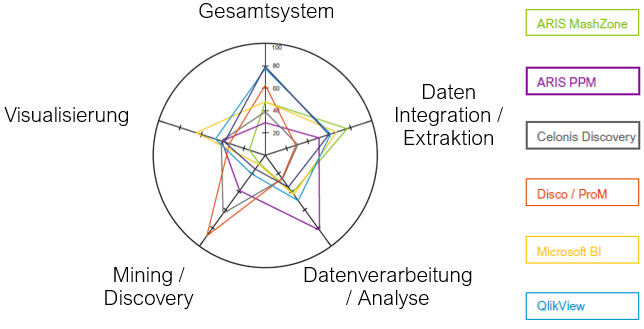
\includegraphics[scale=0.6]{figures/Appbildungen/toolEval.PNG}
    \caption{Bewertung von Process Mining Software (eigene Darstellung in Anlehnung an: J. Schobel, M. Reichert, 2017, S.244, \cite{Schobel2017})}
    \label{fig:toolEval}
\end{figure}
\newpage
Neben der Bedienfreundlichkeit und dem Funktionsumfang sind die ausschlaggebenden Kriterien für die Auswahl der Software jene technischen Daten, die sich direkt auf die praktische Umsetzbarkeit der Testreihe und des Proof of Concept auswirken. Die technischen Eckdaten wurden einer Abschlussarbeit mit dem Titel "Vergleich und Evaluation von Process Mining Software" der Universität Passau entnommen \cite{compPM} und in Tabelle \ref{comparison2} zusammengefasst.

\begin{table}[!h]
\centering
\resizebox{\textwidth}{!}{%
\begin{tabular}{lccc}
\hline
Kriterium & \multicolumn{1}{c}{\textbf{ProM (V. 6.9)}} & \multicolumn{1}{c}{\textbf{Disco }} & \multicolumn{1}{c}{\textbf{Celonis}} \\
\hline\hline
\textit{Typ des Eingangslogs} & Mxml,xes & Csv,xls,XES,xml, fxl & Csv,Xls,XES \\
\textit{Process Discovery} & Ja & Ja & Ja \\
\textit{Lizenz} & Quelloffen & Kommerziell & Kommerziell \\
\textit{Notation der Ergebnisse} & BPMN, PNML, YAWL, PTML & XML & BPMN \\
\textit{Visualisierung der Prozesse} & Ja & Ja & Ja \\
\textit{lokale Anwendung} & Ja, Client-basiert & Ja, Client-basiert. & Nein, Cloud-basiert \\
\textit{Kommandozeilenanbindung} & Ja & Nein & Nein \\
\hline
\end{tabular}%
}
\caption{Gegenüberstellung von technischen Eigenschaften der populärsten Process Mining Lösungen(Quelle: Erling C., Vergleich und Evaluation von Process Mining Software, 2019, S. 36,37,44,83 [\ref{comparison2}])}
\label{comparison2}
\end{table}

Ein entscheidender Vorteil von ProM ist, dass einige der integrierten Plugins eine Kommandozeilenschnittstelle bieten. Mit Hilfe dieser kann die Auswertung der Eventlogs von einem serverseitigen Skript aus gestartet und überwacht werden. Nachteilig an dieser Lösung ist allerdings, dass ProM im Gegensatz zu Disco und Celonis Eventlogs im CSV-Format (\textit{Comma Seperated Values}) nicht direkt entgegen nimmt. Das bedeutet, es muss eine Konvertierung in das XES Format stattfinden, bevor eine Process Mining Analyse durchgeführt werden kann.

Die quelloffene Lizensierung von ProM, die teils Cloud-basierte Architektur von Celonis und der Mangel einer Kommandozeilenanbindung von Disco sind ausschlaggebend für die Entscheidung, ProM als Werkzeug für die Durchführung des Process Mining in dieser Arbeit zu nutzen. 

\subsection{Wahl des Process Mining Verfahrens}
Es soll ein Process Mining Verfahren identifiziert werden, das unter den in den Vergleich einbezogenen Minern am besten geeignet ist Modelle derart zu erzeugen, dass sie kurze, häufig auftretende Ereignisse und Aktionen korrekt erkennen und abbilden. 

Mining Verfahren, deren Modelle zwar korrekt, aber zu komplex sind um eine für den Anwender leicht interpretierbare Regel zu beschreiben sind für diesen Anwendungsfall ungeeignet. In Anbetracht der im Grundlagenkapitel erläuterten Gütekriterien (\ref{sec:quality}) werden hier Modelle gefordert, die ein hohes Maß an ‚Simplicity‘ (Einfachheit) mitbringen und weniger Gewicht auf ,Generalization' legen, also kein Modell erstellen, das dazu neigt alle möglichen, selten auftretenden Prozesschritte mit einzuschließen. 

Ein weiterer Faktor, der die Auswahl an Minern einschränkt, ist die praktische Umsetzbarkeit in einer realen Anwendung. Es werden nur solche Miner berücksichtigt, für die zum Zeitpunkt dieser Arbeit ein Plugin in der ProM-6.9-Version angeboten wird und die in der Lage sind, über Kommandozeilenbefehle so aufgerufen zu werden, dass sie ein Ausgabemodell erzeugen. Das Ziel ist, einen automatisiert ablaufenden Dienst einzurichten, so dass Process Mining ohne zusätzliche Intervention seitens des Anwenders durchgeführt werden kann.

In ProM stehen Plugins des Heuristic, Local, Inductive und des Transitions System Miner zur Verfügung, die diese Anforderung erfüllen. Um beurteilen zu können, welches der Verfahren sich besonders für die Analyse von Eventlogs eignet, die menschliches Verhalten protokollieren, werden Veröffentlichungen herangezogen, die Process Mining im Activities of Daily Living Kontext eingesetzt haben. Die Ergebnisse sind in Tabelle \ref{tab:miningPaper} gelistet. 

Der Local Process Miner ist in der Übersicht nicht aufgeführt, da es bisher keine Veröffentlichungen gibt, die dieses noch junge Verfahren in einem vergleichbaren Kontext eingesetzt haben. 

\newcolumntype{b}{X}
\newcolumntype{s}{>{\hsize=.7\hsize}c}
\begin{table}[!ht]\small
\centering
\begin{tabularx}{\textwidth}{b ccc}
\hline
Titel                                                                                                               & \multicolumn{1}{l}{\textbf{Heuristic}} & \multicolumn{1}{l}{\textbf{Inductive}} & \multicolumn{1}{l}{\textbf{Transition}} \\ \hline\hline
\textit{Discovering process models of activities of daily living from sensors} \cite{adl1}                                      & x                                      &                                        &                                         \\
\textit{Context-based similarity measure on human behavior pattern analysis} \cite{adl2}                                        & x                                      &                                        &                                         \\
\textit{Mining insights from weakly-structured event data} \cite{adl3}                                                          & x                                      & x                                      &                                         \\
\textit{A novel human autonomy assessment system} \cite{adl4}                                                                   &                                        &                                        & x                                       \\
\textit{SAMDY–Technologies to support “Care On Demand”} \cite{adl5}                                                              &                                        &                                        & x                                       \\
\textit{Mining process model descriptions of daily life through event abstraction} \cite{adl6}                                  &                                        & x                                      &                                         \\
\textit{Recompiling learning processes from event logs} \cite{adl7}                                                             &                                        & x                                      &                                         \\
\textit{Event Abstraction for Process Mining Using Supervised Learning Techniques} \cite{adl8}                                  &                                        & x                                      &                                         \\
\textit{Visual process maps: a visualization tool for discovering habits in smart homes} \cite{adl9}                            &                                        & x                                      &                                         \\
\textit{Data Mining for Behavioural Changes and Monitoring Requirements in Residential} Healthcare \cite{adl10}                  & x                                      &                                        &                                         \\
\textit{Prozess-Mining und Prozessbewertung zur Verbesserung klinischer Workflows im Umfeld bilderzeugender Fächer} \cite{adl11} & x                                      &                                        &                                         \\ \hline

\end{tabularx}

\caption{Übersicht über Veröffentlichungen mit dem Thema Process Mining und ADL und das jeweils eingesetzte Process Mining Verfahren}
 \label{tab:miningPaper}
\end{table}
\normalsize
Betrachtet werden hier diejenigen Studien, die eines der Process Mining Algorithmen eingesetzt haben, für das ein Plugin in ProM 6.9 existiert, welches sich über eine Kommandozeilenanbindung ansprechen lässt. Ein weiteres Kriterium war, dass in der Kurzfassung der Veröffentlichung die Absicht beschrieben wurde Daten, die menschliches Verhalten widerspiegeln, über Process Mining zu analysieren. Die Suche erfolgte über die Suchmaschine Google Scholar, die gesuchten Begriffe waren eine Kombination der Bezeichnung des jeweiligen Verfahrens und den Begriffen "ADL", "Smart Home", "Smart Living", "Human Activities" und "Human Behaviour". 

Es lässt sich ein eindeutiger Trend beobachten, der zeigt, dass sowohl der Heuristic als auch der Inductive Miner jeweils ein vergleichsweise populäres Mittel sind, um Protokolldateien, die menschliches Verhalten enthalten, auszuwerten, während der Transitions Miner weniger Beachtung findet. Zusätzlich sollen einige Eckdaten zu den Stärken und Schwächen der Verfahren betrachtet werden, wie sie in Tabelle \ref{tab:my-table} aufgeführt sind. Die Informationen wurden den Veröffentlichungen entnommen, die das jeweilige Verfahren vorstellen (Heuristics \cite{heurMining}, Transitions\cite{transMiner}, Inductive \cite{inducIMining}, Local \cite{localMining}). 

\begin{table}[!h]
\centering
\resizebox{\textwidth}{!}{%
\begin{tabular}{lcccc}
 Kategorie & \textbf{Heuristic} & \textbf{Transitions} & \textbf{Inductive} & \textbf{Local}   \\
%Betrachtete Plugin Version & F. Mannhardt, Interactive Data Aware Heur. M. & H.M.W. Verbeek, Mine for a fuzzy Model & S.J.Leemans, Mine with Inductive Visual Miner & N.Tax, Search for Local Process Models \\
\hline\hline
Nebenläufigkeit & + & - & + & + \\
kurze Iterationen (Schleifenlänge ≤ 2) & + & + & - & + \\
Eignung für unvollständige &  &  &  &  \\
Eventlogs & + & + & + & + \\
Eignung für fehlerbehaftete &  &  &  &  \\
Eventlogs & + & + & ? & ? \\
automatisierbar & + & + & + & +\\
\hline
\end{tabular}%
}
\caption{Eigenschaften von Process Mining Verfahren zur Beurteilung ihrer Eignung für den Einsatz im Smart Home}
\label{tab:my-table}
\end{table}

Die Beschaffenheit der Miner und vorrangig der Trend, der in Tabelle \ref{tab:miningPaper} zu erkennen ist, wurde als hinreichende Bewertungsgrundlage angenommen, um den Heuristic Miner und den Inductive Miner zu wählen und sie in einer Testreihe einem Vergleich zu unterziehen. 

\subsection{Generieren von Protokolldateien}
Um zu untersuchen, inwieweit die Ausgabemodelle der gewählten Miner sich für den im Rahmen dieser Arbeit geplanten Anwendungsfall eignen, werden Protokolldateien benötigt, die menschliches Verhalten beschreiben, welches kurze und regelmäßige Abläufe enthält. Die Protokolldateien werden durch ein im Rahmen dieser Arbeit entstandenes Python Programm generiert, das im Anhang zu einzusehen ist \ref{lst:generate}.

Aufgrund der nahezu unbegrenzten Anzahl möglicher Szenarien, in einem Smart Home durch Protokolldateien aufgenommen werden könnten, kann hier nur ein Ausschnitt simuliert werden. Um dennoch eine hohe Aussagekraft der Testreihe zu erhalten, werden die Eventlogs derart gestaltet, dass sie gegenüber dem Miner inkrementell komplexer werden und so Performanzunterschiede zwischen den Algorithmen sichtbar werden können. 

Der Grad der Abweichung zwischen gesuchtem Modell und der Ausgabe des jeweiligen Miners soll als Grundlage für die Bewertung dienen.

Hervorzuheben ist an dieser Stelle, dass die Miner den Inhalt einzelner Einträge nicht deuten, sie unterscheiden die Ressourcen, die den Eintrag erstellen und die zugehörigen Eigenschaften nur Anhand der Zeichenkette im Protokoll. Dementsprechend werden die Namen der IoT Ressourcen und ihrer Aktivitäten hier zwar beispielhaft für gängige vernetzte Geräte gewählt, sie haben allerdings keine direkte Auswirkung auf das Ergebnis des Mining Verfahrens und sind beliebig austauschbar. Signifikant für die Auswertung ist zunächst nur die Häufigkeit, mit der eine Ressource einen Eintrag erstellt, und der Zeitpunkt des Eintrags im Protokoll, der zu dieser Ressource gehört.

Um eine Vergleichbarkeit mit realen Eventlogs zu ermöglichen, wurden die Eventlogs um Rauscheinträge ergänzt, welche jeweils in ihrem relativen Anteil zur gesamten Protokolldatei variieren. Außerdem variiert die Zeitspanne, die simuliert, wie lange das menschliche Verhalten aufgezeichnet wurde. Eine erfolgreiche Auswertung durch einen Miner hat stattgefunden, wenn das im Ereignisprotokoll eingebettete Muster vollständig im Modell wiedergegeben wird, parallele Abläufe korrekt dargestellt werden und keine überschüssigen (Rausch-) Einträge als Knoten im Ausgabemodell enthalten sind.

Das Programm zur Erzeugung der Eventlogs nimmt folgende Parameter entgegen: das eingebettete, zu erkennende Verhaltensmuster, die Menge an konsekutiven Kalendertagen (30 o. 90 Tage) und den Anteil an Rauscheinträgen (15 o. 50). 

Die Testreihe setzt sich aus zwölf verschiedenen Mustern zusammen. Da es pro gesuchtes Muster vier Kombinationsmöglichkeiten aus Parametern gibt, entstehen insgesamt 48 Protokolldateien, die Aufnahmen aus einem Smart Home simulieren. Die Testreihen tragen jeweils die Namen der Muster („A“ - „M“), insgesamt sind 104 einzelne Wenn-Dann Regeln in den Mustern enthalten, pro Testreihe sind maximal vier dieser Regeln eingebettet. Die Regeln sind in einer Übersicht im Anhang (\ref{sec:config}) einsehbar. 

\section{Bewertungskriterien und Durchführung der Testreihe}\label{sec:tests}
Die Durchführung der Testreihe beinhaltet, jedes der zuvor generierten Eventlogs mit dem Heuristics Miner und dem Inductive Miner auszuführen und das Ergebnis zu protokollieren. Um die Güte der Modelle, die in der Messreihe mit den verschiedenen Minern entstanden sind, zu evaluieren, werden die Ausgaben der Process Mining Plugins mit dem ursprünglich eingebetteten Modell verglichen und der Grad der Abweichung für jeden Datensatz dokumentiert. Um die Performanz der Miner zu quantifizieren, wird die Wiedergabe der eingebetteten Muster im Ausgabemodell über ein Punktesystem bewertet. 

Entscheidend für den im Rahmen dieser Arbeit betrachteten Anwendungsfall der automatisierten Regelerkennung im Smart Home ist, dass der Mining Algorithmus in der Lage ist, Rauschen aus dem Modell herauszufiltern und korrekt kurze Pfade und sowie ihre Parallelität zu identifizieren. Für jedes Ausgabemodell wird die Anzahl der korrekt erkannten Elemente (\textit{True Positive}), sowie die fälschlicherweise im Modell enthaltenen Elemente (\textit{False Postive}) und diejenigen Elemente, die nicht im Modell erscheinen, aber erwartet wurden (\textit{False Negative}), notiert. 
Desweiteren sind Ausgabemodelle nur dann für die Weiterverarbeitung verwertbar, wenn die Elemente, die zu unterschiedlichen Regeln gehören, auch auf unterschiedlichen Pfaden im Modell abgebildet werden. Als weitere Metrik in der Testreihe wird daher die Anzahl der korrekt erkannten Pfade im Ausgangsmodell verwendet (\textit{Parallelism}). Wenn das Ausgabemodell mit dem eingebetteten Muster einer Protokolldatei übereinstimmt, erhält der Miner die volle Punktzahl für das jeweilige Ausgabemodell. Die volle Punktzahl je Ausgabemodell entspricht der Anzahl der eingebetteten Regeln in dem Datensatz.

\section{Auswertung der Ergebnisse}\label{sec:res}
Die Durchführung der Testreihe hat gezeigt, dass es signifikante Unterschiede in der Fähigkeit der untersuchten Mining Algorithmen gibt, Abläufe mit vielen kurzen Pfaden zu identifizieren und im Ausgabemodell korrekt wiederzugeben. Lediglich für fünf der zwölf Reihen geben beide Miner das gesuchte Resultat fehlerfrei aus (konkret: A,B,D,E,F), siehe Tabelle\ref{tab1} und Tabelle \ref{tab2} im Anhang. In den sieben Reihen, in denen einer der beiden Miner Plugins fehlerhafte Ausgabemodelle produzierte, handelte es sich in fünf Fällen (aus 16 Eventlogs, Reihen: H,J,K,L,M) um das ‚Inductive Visual Miner Plugin‘, wohingegen das ‚Interactive Data-aware Heuristics Miner‘ Plugin lediglich in zwei Modellen, in allen vier zugehörigen Eventlogs (Reihen C,G), unterlag. Die Auswertung der Testreihe hat auch gezeigt, dass beide Miner gut geeignet sind bis zu zwei Regeln in einem Eventlog zu erkennen. Bei regelmäßigem Auftreten der Regel konnten auch kurze Auswertungszeitspannen und ein hohes Maß an Rauscheinträgen das Ausgabemodell nicht verzerren.

Im Unterschied zum Heuristic Miner Plugin gelang es dem Inductive Miner Plugin nicht, mehr als zwei kurze Regeln, die in die Eventlogs der Testreihen H,J,K,L,M eingebettet waren, korrekt in parallel verlaufende Pfaden zu unterteilen. Stattdessen gab der Miner häufig alle gesuchten Elemente auf einem einzigen Pfad des Petri Netzes aus, es gelang ihm nicht, die Parallelität der gesuchten Abläufe zu identifizieren. 
Aus der Perspektive des Inductive Miner Verfahrens betrachtet lies sich also beobachten, dass es dem Inductive Miner Verfahren hier nicht gelang, einen \textit{XOR Cut}, siehe \ref{sec:inducMiner}, an der Stelle zu setzen, an der mehr als zwei kurze parallele Abläufe beginnen. 

\begin{figure}[!ht]
    \centering
    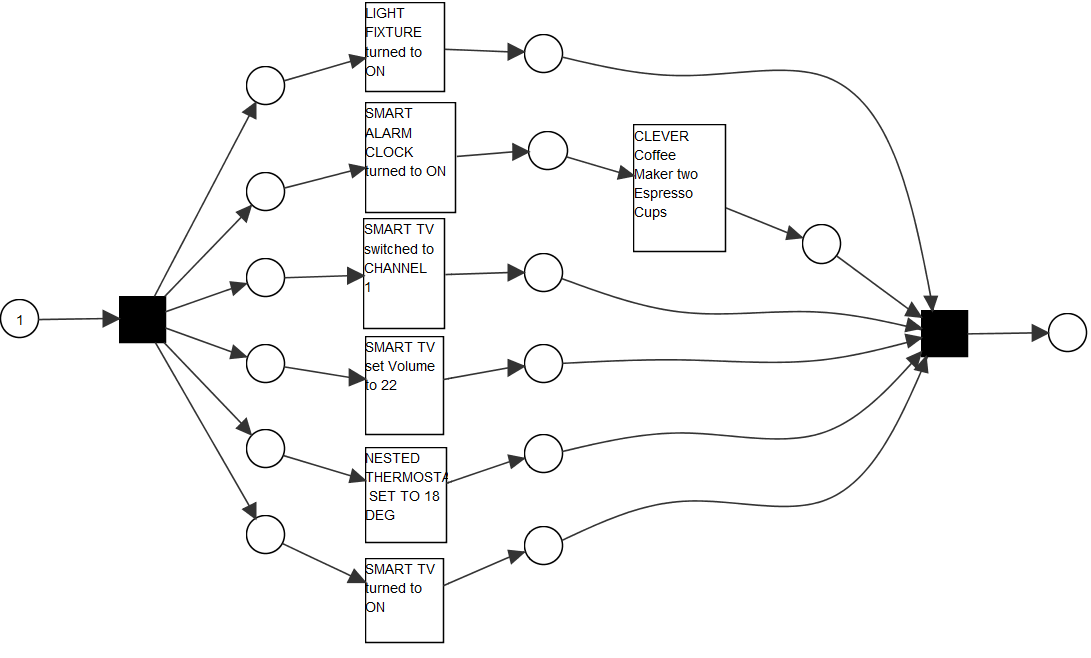
\includegraphics[width=0.9\textwidth,]{figures/Appbildungen/K_inductive_erronousPNG.PNG}
    \caption{Modellierung eines Datensatzes der Testreihe K mit dem Inductive Miner Plugin}
    \label{fig:K_inductive}
\end{figure}
Beispielhaft für diesen Fehlerfall wird das Modell 'K' betrachtet. Eingebettet in die hier eingesetzten Eventlogs lagen drei separate, regelmäßig auftretende Wenn-Dann Abfolgen, bestehend aus jeweils zwei oder drei Elementen. 
Für alle vier Kombinationsmöglichkeiten zur Konfiguration des Eventlogs (30 Tage simulierter Aufnahmezeitraum mit einem Rauschanteil von 15 oder 50 Einträgen und ein Zeitraum von  90 Tagen mit einem Rauschanteil von 15 oder 50) berechnete der Heuristic Miner ein Modell, welches die drei erwarteten Abfolgen enthielt und alle Rauscheinträge herausfiltern konnte, wie in Abbildung \ref{fig:K_heuristic} zu sehen ist.
\begin{figure}[!h]
    \centering
    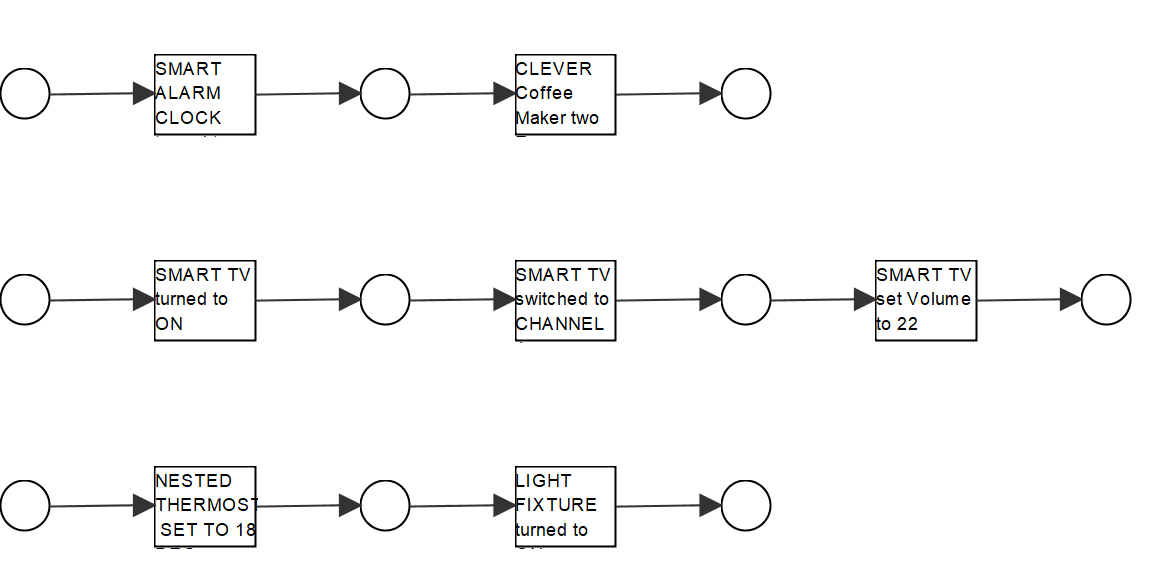
\includegraphics[width=0.8\textwidth,]{figures/Appbildungen/K_heuristic_correct.PNG}
    \caption{Modellierung eines Datensatzes der Testreihe K mit dem Heuristic Miner Plugin}
    \label{fig:K_heuristic}
\end{figure}
Auch das Inductive Miner Plugin war in der Lage das Rauschen herauszufiltern, modellierte aber, bei Eingabe der selben Eventlog Dateien, die das Heuristic Miner Plugin genutzt hat, ein für den Einsatzzweck ungeeignetes Modell. 

Auf Abbildung \ref{fig:K_inductive} ist zu sehen, dass nur eine Regel korrekt in der Wenn-Dann Folge abgebildet wird: auf eine 'Smart Alarm Clock' Aktivität folgt eine 'Coffee Maker' Aktivität. 
Die Komponenten der restlichen eingebetteten Regeln werden zwar erkannt, aber nicht in der korrekten Abfolge, sondern parallel, abgebildet. Diese Form der Abweichung hat sich als charakteristisch für den Inductive Miner herausgestellt. Auch die resultierenden Modelle des Inductive Miner der Reihen H,J,L,M enthielten zwar häufig  die korrekten Elemente, allerdings nicht in der gesuchten Reihenfolge. Es entstanden häufig sogenannte Blumenmodelle, wie sie eingangs beschrieben wurden, siehe Abschnitt \ref{sec:quality}. Die Modellierung fiel also zu allgemein aus, als dass sie gebraucht werden könnte, um in ein If This Then That Schema überführt zu werden.

Auch der Heuristic Miner generierte nicht für jedes Eventlog das erwartete Modell, beispielsweise gelang es ihm in der Testreihe M nicht, alle Rauscheinträge herauszufiltern. Dennoch wurden alle erwarteten Regeln korrekt dargestellt, siehe Abbildung \ref{fig:M_heuristic}. 
Hierbei ist anzumerken, dass die Testreihe M nur an jedem dritten Tag Einträge zum gesuchten Muster enthielt, das heißt das Verhältnis von Rauscheinträgen zu Regeleinträgen war hier besonders hoch, was höchstwahrscheinlich zu der fehlerhaften Modellierung beigetragen hat.
\begin{figure}[!ht]
    \centering
    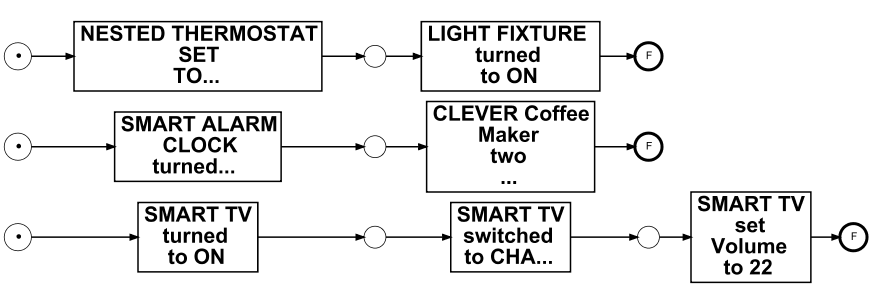
\includegraphics[width=0.7\textwidth,]{figures/Appbildungen/M_Heuristic.PNG}
    \caption{Modellierung der Testreihe M aus dem Heuristic Miner Plugin}
    \label{fig:M_heuristic}
\end{figure}

Aus der Auswertung der Testreihe geht hervor, dass aus insgesamt 104 Regeln, die in den 48 Eventlogs eingebettet wurden, der Heuristic Miner 96 korrekt identifiziert hat, der Inductive Miner hingegen nur in 48 Fällen die gesuchten Regeln korrekt abbilden konnte.

\begin{table}[!htbp]
\centering
\resizebox{\textwidth}{!}{%
\begin{tabular}{l|ccccc}
Auswertung                & \multicolumn{1}{l}{\textbf{Testreihen}} & \multicolumn{1}{l}{\textbf{Regeln}} & \multicolumn{1}{l}{\textbf{Fehlerhafte Modelle}} & \multicolumn{1}{l}{\textbf{Identifizierte Regeln}} & \multicolumn{1}{l}{\textbf{Verfehlte Regeln}} \\ \hline
\textit{Inductive M.}  & 48                                      & 104                                 & 14                                               & 48                                                 & 56                                            \\
\textit{Heuristics M.} & 48                                      & 104                                 & 2                                                & 96                                                 & 8                                            
\end{tabular}%
}
\caption{Ergebnisse der Auswertung der Versuchsreihe}
\label{tab:results_short}
\end{table}

Da ein Verfahren gesucht wurde, das kurze Regeln, also Abläufe bestehend aus zwei bis vier Elementen, erkennt und  in der Lage ist mehrere Regeln, die in einem Eventlog eingebettet sind klar voneinander zu trennen, ging das Heuristic Miner Plugin aus der hier vorgestellten Testreihe als zu bevorzugendes Verfahren hervor.

Neben den Erkenntnissen über die wahrscheinliche Eignung der untersuchten Process Mining Verfahren für den Einsatz zur automatisierten Regelerkennung, konnte außerdem beobachtet werden, welche Parameter, die den Process Mining Verfahren eigen sind, eine positive oder negative Auswirkung auf die Auswertung haben. 

So gibt es beispielsweise die Möglichkeit, dem Heuristic Miner Plugin "all tasks connected", also "Verbinde alle Abläufe" auf \textit{wahr} zu setzen, was konsistent zu Modellen führt, die von Anwendern und Entwicklern des Process Mining gemeinhin als ,Spaghettimodell' bezeichnet werden, wie es hier für einen Datensatz der Testreihe A in Abbildung \ref{fig:A_heuristic_spagh} zu sehen ist.
\begin{figure}[!ht]
    \centering
    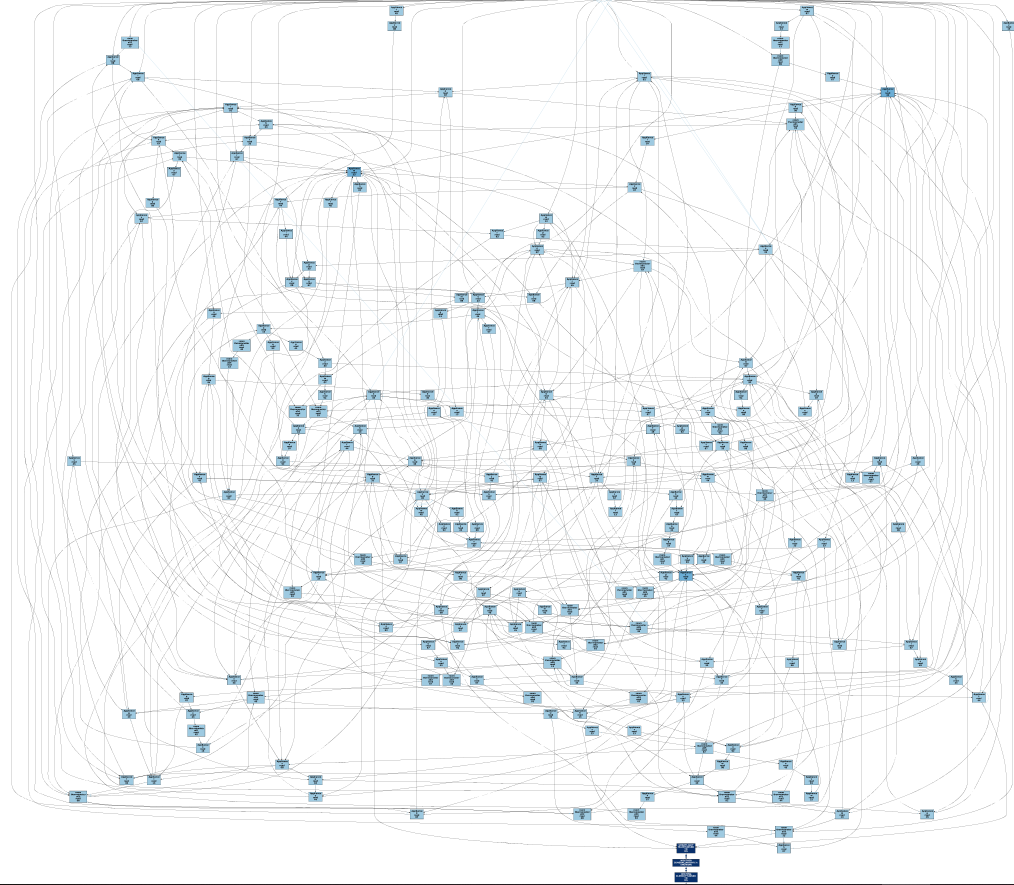
\includegraphics[width=0.65\textwidth,]{figures/Appbildungen/A_underfitted.PNG}
    \caption{Modellierung der Testreihe A aus dem Heuristic Miner Plugin}
    \label{fig:A_heuristic_spagh}
\end{figure}

Basierend auf den Erkenntnissen dieser Testreihe wurde das Heuristic Miner Plugin gewählt, um ihn für die Konstruktion des Proof of Concept einzusetzen und desweiteren notiert, dass der Parameter "all tasks connected" auf \textit{false} zu setzen ist.
%Desweiteren deutet die Auswertung der Testreihe darauf hin, dass der Einsatz des Heuristic Miners möglicherweise Prinzipiell gegenüber dem Inductive Miner zu bevorzugen ist, wenn nach einer Modellierung gesucht wird, die dem If This Then That Schema entspricht, also Muster enthält, die jeweils aus mehreren Ketten besttenur wenigen aufeinanderfolgenden Elementen bestehen.





%\Rotatebox{90}{%
%\centering
%    \begin{tabular}{lp{2cm}p{2cm}p{2cm}p{2cm}p{2cm}p{2cm}}
%& Alpha Miner & Heuristic Miner & Heuristic Miner + & Fuzzy %Miner & Transition System Miner & Transition System Miner + %\\
%(garantierte) Ausführbarkeit & - & ? & ? & - & + & + \\
%Nebenläufigkeit & + & + & + & - & + & + \\
%Intervalle & - & - & + & - & + & + \\
%kurze Iterationen (Schleifenlänge ≤ 2) & - & + & + & + & + & %+ \\
%entfernte Abhängigkeiten/ nicht lokales Verhalten & - & + & + %& + & + & + \\
%nicht wahrnehmbare Aktivitäten & - & + & + & - & + & + \\
%Eignung für unvollständige Event Logs & - & + & + & + & + & + %\\
%Eignung für fehlerbehaftete Event Logs & - & + & + & + & - & %- \\
%Frequenz von Traces wird berücksichtigt & - & + & + & ? & - & %+ \\
%parametrisierbar & - & + & + & + & + & + \\
%automatisierbar & + & - & - & - & - & + \\
%tolerant gegenüber unstrukturierten Prozessen & - & ? & ? & + %& - & - \\
%ein Mining-Schritt & + & + & + & + & - & - \\
%zwei Mining-Schritte & - & - & - & - & + & + \\
%Ausgabeformat & & & & & & \\
%Petri-Netz & + & - & - & - & + & + \\
%heuristisches Netz & - & + & + & - & - & - \\
%Fuzzy-Modell & - & - & - & + & - & - \\
%Transitionssystem & - & - & - & - & + & + \\
%\end{tabular} 
%}

%\begin{table}[h!]
%\centering
%\begin{tabular}{ccccccc}
%& Alpha Miner & Heuristic Miner & Heuristic Miner + & Fuzzy Miner & Transition System Miner %& Transition System Miner + \\
%(garantierte) Ausführbarkeit & - & ? & ? & - & + & + \\
%Nebenläufigkeit & + & + & + & - & + & + \\
%Intervalle & - & - & + & - & + & + \\
%kurze Iterationen (Schleifenlänge ≤ 2) & - & + & + & + & + & + \\
%entfernte Abhängigkeiten/ nicht lokales Verhalten & - & + & + & + & + & + \\
%nicht wahrnehmbare Aktivitäten & - & + & + & - & + & + \\
%Eignung für unvollständige Event Logs & - & + & + & + & + & + \\
%Eignung für fehlerbehaftete Event Logs & - & + & + & + & - & - \\
%Frequenz von Traces wird berücksichtigt & - & + & + & ? & - & + \\
%parametrisierbar & - & + & + & + & + & + \\
%automatisierbar & + & - & - & - & - & + \\
%tolerant gegenüber unstrukturierten Prozessen & - & ? & ? & + & - & - \\
%ein Mining-Schritt & + & + & + & + & - & - \\
%zwei Mining-Schritte & - & - & - & - & + & + \\
%Ausgabeformat & & & & & & \\
%Petri-Netz & + & - & - & - & + & + \\
%heuristisches Netz & - & + & + & - & - & - \\
%Fuzzy-Modell & - & - & - & + & - & - \\
%Transitionssystem & - & - & - & - & + & + \\
%\end{tabular} 
%\caption{Eigenschaften der wichtigsten Mining Algorithmen}
%\label{table:1}
%\end{table}
    \chapter{Proof of concept, praktische Anwendung}\label{chap:experiments}
Die lokale Auswertung persönlicher Daten ist das Hauptargument für eine dezentralisierte Smart Home Steuerung aus Sicht von Konsumenten, die, wie in der Befragung des IDC einsehbar \cite{IDC}, häufig angeben, dass die mögliche Auswertung ihrer Informationen durch Dritte ein ausschlaggebender Faktor gegen die Anschaffung eines solchen Systems darstellt. 
Der Aufbau dieser Anwendung sieht daher vor, die Datenanalyse vollständig innerhalb des Heimnetzes des Anwenders durchzuführen, sich also auf eine „Small Data“ Analyse zu beschränken und so den Einwänden, die mit „Big Data Mining“ einhergehen, vorzugreifen. 

Um den theoretisch skizzierten Anwendungsfall praktisch zu untersuchen, wird der gewählte Process Mining Algorithmus auf einem einfachen, im lokalen Netz erreichbaren, Server als Dienst implementiert. Dieser wartet auf das Eintreffen von Eventlogs aus einem Smart Home, verarbeitet die Rohdaten und leitet das resultierende Modell an eine mobile Anwendung weiter. Die Anwendung soll dem Bewohner die Möglichkeit geben, die vom Process Mining Algorithmus extrahierten Regeln im Smart Home zu integrieren. Wird die Regel vom Bewohner akzeptiert, übernimmt der lokale Server die Automatisierung der Abläufe auf den relevanten vernetzten Geräten.

\section{Aufbau und Komponenten der praktischen Anwendung}
Das Smart Home Modell, das zu Testzwecken in dieser Arbeit dient, wird vom ITOM Institut der FH Aachen betrieben und ist mit unterschiedlichen Sensoren und Aktoren ausgestattet. 
Außerdem wird die Android Anwendung „Grafischer Regeleditor“, die zuvor im Rahmen einer Abschlussarbeit am ITOM Institut entstandenen ist, als Grundlage für die Kommunikation mit dem Anwender genutzt und um die Funktion der automatisierten Regelerkennung erweitert. 
Die Funktionalität der Kommunikation mit einem lokalen Server und das manuelle Anlegen von Regeln für IoT Geräte ist bereits in der Anwendung integriert.

Die Auswertung durch das Process Mining, die Archivierung der Eventlogs und die Kommunikation mit den vernetzten Geräten des Smart Homes werden von einem einfachen Server mit ARM-Prozessor übernommen, konkret handelt es sich dabei um ein Raspberry Pi 3.0. Um den Anwender über neue erkannte Muster zu informieren, wird jeweils eine Benachrichtigung an das Mobiltelefon versandt. Das Versenden der Benachrichtigung übernimmt der \textit{firebase}\footnote{https://firebase.google.com/} Dienst. Diese Aufgabe könnte, um den Aspekt des Datenschutzes voll zu erfüllen, ebenfalls von einem lokalen Dienst durchgeführt werden.

\section{Dienste und Skripte auf dem Heimserver}
Da die Anwendung auf der Architektur des Projekts „Grafischer Regeleditor“ aufbaut, wird in dieser Arbeit vorausgesetzt, dass openHab als Dienst im Heimnetzwerk des Anwenders eingerichtet ist. Dieser Dienst ist eine essentielle Komponente der Anwendung, er ist verantwortlich für die Kommunikation mit den IoT Geräten. Sowohl die Erzeugung der Protokolldatei als auch die Ausführung von Regeln erfolgt mithilfe von openHab. 

Die quelloffene openHAB (open Home Automation Bus) Automatisierungssoftware implementiert eine weite Bandbreite herstellerabhängiger Standards und gewährleistet so die Kommunikation zwischen unterschiedlichen vernetzten Geräten. Die Automatisierungslogik der openHAB-Software ist als einfacher Regex-Agent anzusehen. 
Um die Brücke von der unverarbeiteten gesammelten Menge an Ereigniseinträgen zu einer neuen, automatisiert erkannten Regel zu schlagen wird ein Skript auf dem Server hinterlegt, welches periodisch alle notwendigen Verarbeitungsschritte des Prozesses aufruft. In regelmäßigen Abständen wird das auf dem lokalen Server hinterlegte Eventlog geladen und zunächst vom CSV in das XES Format konvertiert. 

Diese Konvertierung ist ein simpler Vorgang, bei dem jeder Eintrag, der in der CSV Datei eine einzelne Instanz einer Aktion eines IoT Geräts repräsentiert, in seine Komponenten teilt und in das XES Format übertragen wird. Die Komponenten umfassen, wie in Abschnitt \ref{sec:xes} beschrieben, den Zeitstempel, den Namen des Geräts - in der Form in der er unter openHab hinterlegt ist - sowie die Aktion oder den Sensorwert der den Eintrag erzeugt hat. Die einzelnen Komponenten werden im Ausgangsformat von XML-Tags eingeschlossen. Dieser Schritt ermöglicht die Verarbeitung der Daten mit ProM.

%Bei der Untersuchung von unverarbeiteten Eventlogs, die im Smart Living Modellhaus des ITOM Institus entstanden sind, ist erkennbar, dass es bei einigen der im Haus integrierten Geräte dazu kommt, dass sie ein Zeitstempelformat nutzen, welches die Sekunden nicht angibt. Hier ist also vor der Konvertierung ein Vorverarbeitungssschritt notwendig, der über jede Zeile iteriert und die Stempel einander angleicht. Da kein universeller Standard für IoT Logs Branchenweit akzeptiert wird und die Hersteller diese beliebig formatieren können, sind mit jedem weiteren angeschlossenen Gerät auch weitere Abweichungen von der erwarteten Form nicht auszuschließen. Um diesem Problem entgegenzuwirken können Tools wie ‚syslog-ng‘ eingesetzt werden, die in der Lage sind die meisten Formen von Eventlogs auf ein einheitliches Format zu bringen.

Im nächsten Schritt ruft das Skript ein in der Programmiersprache Java geschriebenes Programm auf, welches Process Mining auf dem neu entstandenen XES Dokument durchführt. Konkret wird dafür ProM auf dem Server gestartet und das Heuristic Miner Plugin ausgewählt.
Über Parameter kann die Analyse durch das Heuristic Miner Plugin zusätzlich angepasst werden, etwa um Rauschdaten zu unterdrücken oder weitere Attribute bei der Datenanalyse zu berücksichtigen, falls diese im Eventlog gegeben sind. Der Vorverarbeitungsschritt der Rauschreduzierung ist unerlässlich für die Regelfindung. Es sollten keine Knoten als Teil des Regelvorschlags an den Nutzer gelangen, die nicht auch Teil seines regulären Ablaufs sind. 


In dieser Arbeit wird der Schwellwert für Rauschdaten über einen iterativen Prozess gesucht. Da es im Vorfeld keine Information über die Menge der Rauschdaten im zu untersuchenden Eventlog geben kann, wird wie folgt verfahren. 

\begin{figure}[!h]
    \centering
    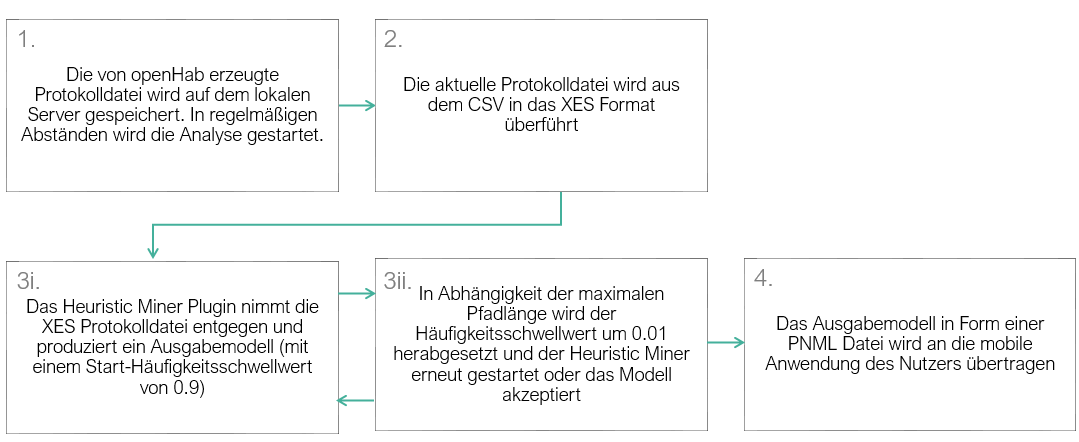
\includegraphics[width=\textwidth,origin=c]{figures/Appbildungen/ServerSchritte.PNG}
    \caption{Verarbeitungsschritte zur Auswertung der Smart Home Daten auf dem Server}
    \label{fig:server}
\end{figure}

\newpage
Ziel ist es ein Modell der häufigsten, kurzen Routinen zu finden. Genauer soll eine Regel mindestens eine Vorbedingung und eine Aktion enthalten, maximal drei Vorbedingungen werden akzeptiert. Nachdem ein Modell aus zwei Knoten gefunden wurde, wird dieses um einen weiteren Knoten erweitert, wenn die Auftrittshäufigkeit des Elements mindestens so hoch ist wie die bisherigen Elemente. Der Regler für den Häufigkeitsschwellwert (im Plugin 'frequency' genannt) wird mit einem Startwert von 0.9 initialisiert, ein Petri Netz erzeugt und dessen Knoten gezählt. Der Schwellwert wird inkrementell (Schritte von 0.1) verringert, bis eine Veränderung im Ausgabemodell auftritt. Ist die Auftrittshäufigkeit des neuen Elements im Ausgabemodell im Vergleich zum Vorangegangen geringer, wird das Vorgängermodell als korrekte Regel akzeptiert. Liegt die Auftrittshäufigkeit auf dem selben Niveau, wird der Wert weiter dekrementiert, bis sich das Modell verändert. Tritt ein weiterer Eintrag im Ausgabemodell auf, wird wieder die Auftrittshäufigkeit verglichen. Dieser Vorgang wird wiederholt, bis maximal drei Vorbedingungen eine Regel bilden oder die Auftrittshäufigkeit des neuen Eintrags unter dem der anderen Einträge liegt.

Ist dieser Prozess abgeschlossen, ist eine Regel gefunden worden.
Das Modell des Miners wird zunächst im PNML Format gespeichert, welches Petri Netze nach dem XML Schema beschreibt. Das Petri Netz wird dann in ein If This Then That Schema überführt.

Abschließend enthält das Skript einen Aufruf an ein kurzes, in Python geschriebenen Programmm, welches den Firebase Dienst dazu auffordert eine Benachrichtigung an das mobile Gerät des Anwenders zu senden, welche den Inhalt des neuen Dokuments übermittelt. Der Prozess, der auf dem Server stattfindet, ist in wenigen Schritten auf Abbildung  \ref{fig:server} dargestellt.

\section{Mobile Anwendung als Steuerungs- und Kommunikationsschnittstelle}

Um die Regeleditor Anwendung um die Kommunikation mit einem dedizierten Firebase Dienst zu erweitern, wird eine Klasse PMFireBaseMessagingService angelegt. Diese ist dafür verantwortlich, die Regel entgegenzunehmen und übergibt sie an die im Rahmen dieser Arbeit erzeugte \textit{PMRule} Klasse, die verantwortlich für die Überführung der empfangenen Nachricht in eine Regelform ist. Konkret wird dies von der Funktion parseReceivedRule() übernommen.
\small
\begin{lstlisting}[language=Java]
       private void parseReceivedRule(JSONArray ruleJSON) throws JSONException {
        PMRule r = new PMRule();
        int lastEntry = 0 ;
        for(int j=0;j<ruleJSON.length();j++){
            Log.d("processmining", "rules Array"+j+": "+ruleJSON.getJSONArray(j));

            if(ruleJSON.getJSONArray(j).length()>1){
                lastEntry = ruleJSON.getJSONArray(j).length()-1;
                Vector<String> preconditions = new Vector<>();
                for(int i=lastEntry; i>=0;i--){
                    if(i==lastEntry)
                        r.setAction(ruleJSON.getJSONArray(j).getString(i));
                    else
                        preconditions.add(ruleJSON.getJSONArray(j).getString(i));
                }
                r.setPrecondition(preconditions);
                PMRules.add(r);
                Log.d("processmining", "IF: "+r.getPrecondition()+" THEN: "+r.getAction());
            }
        }
        Intent pmIntent = new Intent(Main.this, ProcessMiningRuleActivity.class);
        pmIntent.putExtra("IF", r.getPrecondition());
        pmIntent.putExtra("THEN", r.getAction());
        startActivity(pmIntent);
    }
\end{lstlisting}

\begin{wrapfigure}{R}{0.5\textwidth}
  \begin{center}
    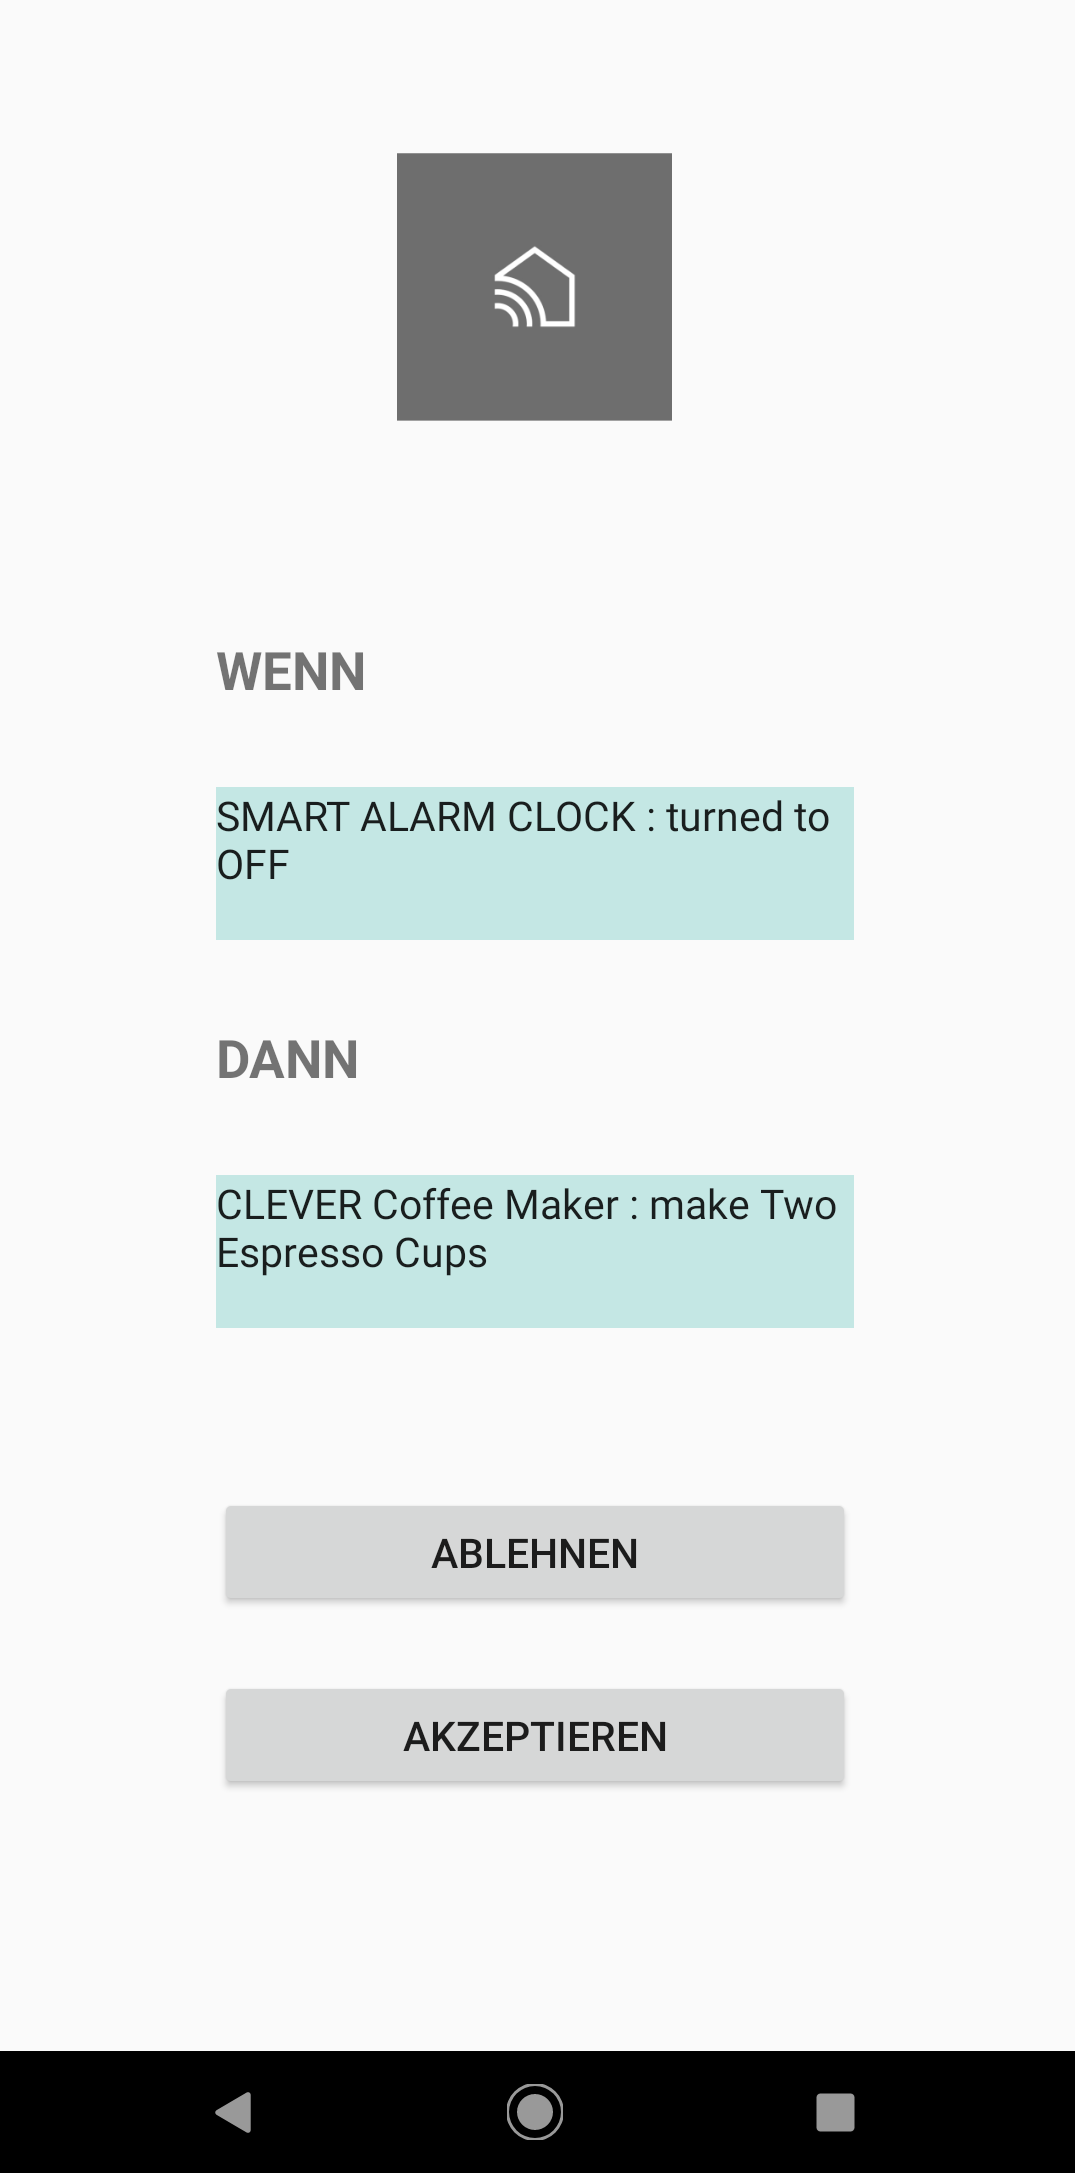
\includegraphics[width=0.3\textwidth]{figures/Appbildungen/newRuleDialog.png}
  \end{center}
  \label{fig:dialog}
  \caption{Proof of Concept: Dialog bei Eingang neuer erkannter Regel}
\end{wrapfigure}
\normalsize

Diese Funktion erlaubt das klassifizieren der Elemente in Vor- und Nachbedingungen, die dann direkt in die vorhandene Datenbank der Anwendung "Grafischer Regeleditor" eingefügt werden können.

Durch die Benachrichtigung, die auf dem Mobilen Gerät angezeigt wird, wenn der Firebase Dienst eine neue Regel zugestellt hat, wird ein Dialog innerhalb der „Grafischer Regeleditor“ Anwendung gestartet. Ein Beispiel für den Dialog ist auf Abbildung \ref{fig:dialog} zu sehen. Die Vorbedingungen und Aktionen der Regel werden im Wenn – Dann Format dargestellt. Der Nutzer hat zunächst die Möglichkeit die Regel zu akzeptieren oder abzulehnen. Wird sie abgelehnt, wird die Regel nicht ins lokale openHab System aufgenommen und eine entsprechende Feedback Nachricht an den Server übermittelt. Dieser Schritt soll verhindern, dass eine vom Anwender nicht erwünschte Regel wiederholt vorgeschlagen wird. Der Server soll neue Regeln zunächst gegen bestehende und abgelehnte Regeln abgleichen, bevor eine neue Anfrage an den Benutzer gestellt wird.

Wird der Vorschlag vom Anwender akzeptiert, wird er zu einem weiteren Fenster weitergeleitet, welches ihm die Option bietet, die Regel ohne Anpassungen zu übernehmen, oder aber die vorgeschlagene Regel zu editieren. Beispielsweise können weitere Vorbedingungen oder Aktionen hinzugefügt oder entfernt werden. 


Für diese Funktionalität wird auf das Regelwerk der zur Verfügung gestellten „Grafischer Regeleditor“ App zurückgegriffen. 

Nachdem die Regel vom Nutzer akzeptiert worden ist, wird sie wie in der Vorgängerversion der Anwendung auch in eine SQLite Datenbank eingetragen. OpenHab empfängt die aktualisierten Regeln aus der Datenbannk und wird nun die Aktion ausführen, sobald die vermerkten Vorbedingungen erfüllt sind.
Weitere Funktionen wie das nachträgliche Entfernen oder Editieren der Regeln stehen dem Anwender wie bereits in der Vorgängerversion zur Verfügung.
Der clientseitige Prozess wird in Abbildung \ref{fig:Kommunikationsablauf} noch einmal im BPMN Format graphisch dargestellt.
\newpage
\begin{figure}[!ht]
    \centering
    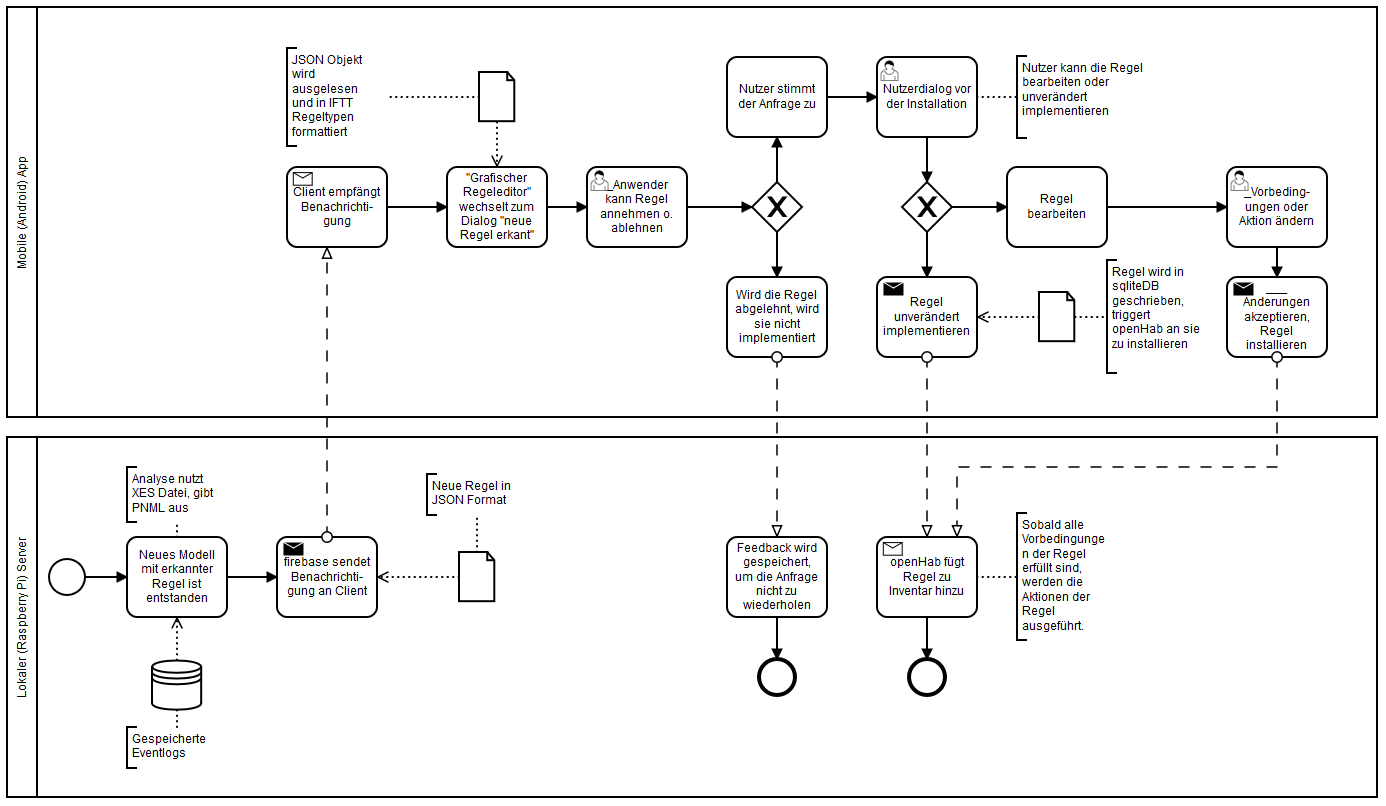
\includegraphics[width= 1.47\textwidth, angle=90,origin=c]{figures/Appbildungen/diagramm_app.PNG}
    \caption{Ablauf der Kommunikation zwischen Endanwender und lokalem Server}
    \label{fig:Kommunikationsablauf}
\end{figure}
    \chapter{Zusammenfassung und Ausblick}
\section{Zusammenfassung}
\vspace{5mm}
\textsl{Ist die automatisierte Erfassung und lokale Verarbeitung von Abläufen im Smart Home durch Process Mining auf lokalen Servern mit eingeschränkter Rechenleistung möglich?}
\vspace{5mm}

Es konnte gezeigt werden, dass Process Mining prinzipiell dazu geeignet ist, mehrere kurze Verhaltensmuster in emulierten Smart Home Protokolldateien zu entdecken. Unter der Voraussetzung, dass die zu analysierende Protokolldatei regulär autretende Abläufe enthält, und diese sich von den anderen Einträgen in ihrer Auftrittshäufigkeit abheben, sind Process Mining Algorithmen in der Lage, diese Abläufe zu entdecken und zu abstrahieren. Diese Beobachtung legt nahe, dass auch Protokolldateien, die aus realen Smart Living Umgebungen stammen, verwendet werden können, um durch Process Mining kurze, repititive Muster zu extrahieren. 

Der Detektionsprozess war auch mit Protokoldateien, die sich nur über kurze Zeiträume erstrecken, in der Lage die erwarteten Abläufe aufzudecken. Selbst die begrenzten Rechenressourcen eines handelsüblichen Einplatinencomputers reichten aus, um eine automatisierte Regeldetektion durchzuführen, und die erkannte Regel über wenige Verarbeitungsschritte an eine Anwendung auf einem mobilen Endgerät zu übermitteln.

Dem Anwender kann potentiell auf diese Weise zeitintensive Konfigurationsarbeit abgenommen werden, so dass gleichzeitig die Bedienfreundlichkeit im Smart Home erhöht wird. In dem vorgestellten Aufbau wurde Rücksicht auf den, in den Eingangs erwähnten Umfragen geäußerten, Wunsch genommen, private Smart Home Daten des Anwenders zur Auswertung nicht an Dritte zu übergeben. Alle Schritte der Hausautomatisierung und Analyse kommen ohne Interaktion mit einer Cloudinfrastruktur aus und können auf Basis von kleinen Datenmengen arbeiten, die automatisierte Regelerkennung kann isoliert innerhalb eines lokalen Netzwerkes ausgeführt werden.

Der Vergleich von aktuell verbreiteten Process Mining Verfahren und Process Mining Software hat gezeigt, dass dieses noch junge Forschungsgebiet bisher vorrangig in der Industrie produktiv eingesetzt wird und dort Antworten auf ökonomisch relevante Fragen liefert. Dementsprechend ist auch die Mehrheit der Softwareanbieter im Bereich des Process Mining auf Anwendungen im betrieblichen Umfeld fokussiert. 
Für die Forschung und andere, nicht industrielle, Einsatzzwecke ist die Process Mining Produktreihe der 'Process Mining Group' an der Uni Eindhoven die bisher einzige Lösung, welche gleichzeitig den erforderlichen Funktionsumfang und die notwendige Flexibilität bietet wie kommerzielle Lösungen. Da ein Großteil der Software, der in der "Process Mining Group" entstanden ist, der Öffentlichkeit lizenzfrei zur Verfügung steht und die Plattform dank Plugins, die von Wissenschaftlern und unabhängigen Programmierern auf dem Gebiet entwickelt werden, stetig wächst, eignet sie sich ideal um neue Anwendungsgebiete für die Process Mining Technologie zu erproben.
Eine Evaluation mit synthetisierten Daten hat gezeigt, dass das Inductive Miner Verfahren und das Heuristic Miner Verfahren fähig sind, kurze Regeln korrekt zu extrahieren. Im Rahmen der Testreihe hat sich weiterhin ergeben, dass der Heuristic Miner besser geeignet war Modelle derart zu konstruieren, dass sie sich in eine If This Then That Struktur überführen lassen. Die Modelle konnten dann in Form von Regeln in die  Hausautomatisierung integriert werden.

Basierend auf diesen Erkenntnissen wurden die Komponenten des Proof of Concept gewählt, welche Gleichzeitig eine Weiterentwicklung eines vorangegangenen Projekts des IT Organisation und Management Institus der Fachhochschule Aachen beinhalten. Es wurde ein Hintergrunddienst umgesetzt, der das Heuristic Miner Verfahren über die Kommandozeilenanbindung der Software ProM auf gesammelten Smart Home Daten anwendet. Diese werden wiederum von einer Android Anwendung in Regeln umgewandelt, die in eine gegebene openHab Umgebung integriert werden können.
\newpage
\section{Ausblick}
Aus der Untersuchung von Process Mining Verfahren im Smart Living Kontext ergeben sich Fragestellungen in zwei Bereichen: in der Forschung des Process Mining im Bereich des \textit{activites of daily living} (ADL) und in der Entwicklung von Smart Home Anwendungen.

\subsection{Entwicklung von Smart Home Anwendungen}
Sinkende Kosten für die Produktion von Sensoren und elektronischen Bauteilen tragen zur rasant wachsenden Verbreitung von vernetzten Geräten bei, wodurch es als wahrscheinlich gilt, dass auch immer mehr einfache Haushaltsgeräte, wie etwa simple Einrichtungsgegenstände, in Zukunft digital vernetzt werden. Die Auswertung von Rohdaten und die Suche nach Mustern in diesen Daten wird durch eine höhere Datendichte erleichtert. Dadurch wächst auch das Potential und die Aussagefähigkeit von Datenanalysen im Smart Living Umfeld.

Denkbar ist auch die Anreicherung der vom Smart Home Daten automatisch erzeugten Datensätze durch weitere Daten des Anwenders, wie Kalendereinträge oder Informationen, die durch andere elektronische Geräte wie etwa Smart Watches, gesammelt werden. Auf diese Weise kann die Bandbreite und Präzision der erkannten Abläufe erhöht, und dem Nutzer so noch individueller zugeschnittene Regeln angeboten werden, die sich dynamisch an Änderungen in dessen Tagesplanung anpassen können.

Die Ergebnisse dieser Arbeit deuten darauf hin, dass der Einsatz von Process Mining prinzipiell dazu geeignet ist, einfache Prozesse aus Eventlogs zu extrahieren, die in einem Smart Home entstehen. Die in dieser Arbeit beschriebene Anwendung profitiert davon, dass die Elemente eines aus dem Process Mining resultierenden Modell fast unverändert und unverarbeitet in die Hausautomatisierungssoftware eingegeben werden können, um einen Mehrwert für den Anwender zu generieren. 

Sollen komplexere Abläufe als Regeln verstanden werden, etwa eine automatisierte Klassifizierung von übergeordneten Handlungen wie beispielsweise „Frühstück zubereiten“, indem mehrere Aktionen und Sensorwerte zu einem zusammenhängenden Prozess vereint werden, ist eine aufwendigere Vorverarbeitung der Daten notwendig. Hier ist absehbar, dass es notwendig ist, Daten durch Metainformationen anzureichern um kontextuelle Abhängigkeiten zwischen verschiedenen Eventlogeinträgen herzustellen, etwa durch Clusteringverfahren. 

Diese Ansätze könnten außerdem genutzt werden, um die Modelle aus Local Process Mining Verfahren zu gewichten und so direkt für die in dieser Arbeit vorgestellten Funktion der automatisierten Regelerkennung einzusetzen. Dies würde auch den Schritt der iterativen Suche nach einem geeigneten Schwellwert im Heuristic Miner Verfahren erübrigen und das Charakteristikum des Local Process Miner, sich auf mehrere kurze Abläufe zu fokussieren, effektiv ausnutzen.

Darüber hinaus könnte der Einsatz des Process Mining im Smart Home insbesondere unterstützend in der Alten- und Krankenpflege eingesetzt werden. Da es durch den demographischen Wandel zu einem akuten Mangel an Pflegekräften kommt, dem aktuell viele technologische Forschungsinitiativen versuchen entgegenzuwirken, wäre eine automatisierte Analyse von Tages- und Pflegeabläufen in Alten- und Pflegeeinrichtungen durch Process Mining möglich. Für dieses Einsatzgebiet gibt es bereits einige wenige Studien, die darauf hinweisen, dass die aus dem Process Mining gewonnen Modelle zur Verbesserung der Abläufe dienen können, beispielsweise um fehlerhaft durchgeführte Prozesse hinzuweisen, sowie dazu beizutragen Aussagen über den Zustand und die Entwicklung von Patienten zu treffen. Auch an dieser Stelle ist davon auszugehen, dass die Auswertung von Daten, die durch Sensoren erfasst werden, welche in der Umgebung der Patienten integriert sind, eine höhere Akzeptanz erfahren, als solche, die durch bildbasierte Methoden wie Überwachungskameras entstehen.

Besonders interessant sind aber auch hier systematische Ansätze, die nicht allein die Rohdaten direkt in Prozessmodelle überführen, sondern kontextuelle Informationen (\textit{Context Awareness}) in die Analyse einbeziehen und über mehrere Eventlogeinträge abstrahieren, so dass das Analyseergebnis insgesamt an Aussagekraft gewinnt.
Werden beispielsweise Temperatur und Herzschlagrate sensorisch erfasst, könnten nicht nur der aktuelle Wert an ein Monitoring System ausgegeben werden, sondern auch eine Hinweis dazu, ob eine Steigung in den Werten auf eine akute Verletzung oder auf sportliche Aktivität zurückzuführen ist.

Aus der Relevanz von Kontextinformationen für das Process Mining und dem Bedarf nach Methoden, diese nicht manuell, sondern systematisch und automatisiert aus Rohdaten zu gewinnen, ergeben sich auch zentrale Forschungsfragen für die Datenanalyse.

\subsection{Forschungsfragen zu Process Mining}
Nicht nur im Bereich des Smart Living, auch in der Industrie wächst die Qualität der Aussagekraft von Modellen unweigerlich durch die Hinzugabe von Metainformationen zu den gegebenen gesammelten Rohdaten. Gleichzeitig ist die manuelle Eingabe solcher Informationen ein zeit- und kostenintensiv Prozess, der zudem fehleranfällig ist, da er auf der menschlichen Beurteilungsgabe beruht.

Die im Rahmen dieser Arbeit eingesetzte Process Mining Analyse ist, wie die allermeisten Process Mining Anwendungen bisher, rein syntaktisch orientiert. Das heißt der Auswertungsprozess von Rohdaten besteht aus Schritten der Datenfilterung und der iterativen Suche nach geeigneten Parametern, bis ein Ergebnis generiert wird, dass eine gegebene Fragestellung hinreichend beantwortet. Process Mining Verfahren differenzieren die Daten, die sie untersuchen aber nicht danach, welchen Inhalt sie widerspiegeln. 

Die Umsetzung der praktischen Anwendung hat außerdem zum Vorschein gebracht, dass das Filtern von ungeordneten Daten, wie jene eines Smart Home, ein Problem darstellen. Nur den Häufigkeitswert zu berücksichtigen führt zu teils unzureichenden Ausgabemodellen, wie es auch die Autoren der Studie "Discovering more precise process models from event logs by filtering out chaotic activities", die in Abschnitt \ref{har} bereits erwähnt wurde, anmerken \cite{Tax2019}. Es ist eine verbesserte Analyse menschlicher Verhaltensmuster durch Process Mining zu erwarten, wenn zunächst die Filterverfahren für die Vorverarbeitung der Daten verbessert werden.
Technologien, die es hingegen ermöglichen, semantische Informationen aus Rohdaten zu extrahieren werden für viele Datenanalyseverfahren gebraucht und entwickelt. Entsprechende Lösungen sind jedoch meist auf das jeweilige Verfahren und die gegebene Fragestellung zugeschnitten und selten auf andere Anwendungsfälle übertragbar. 

Hieraus ergibt sich der Bedarf an verbesserten Verfahren, die es ermöglichen semantisches Process Mining zu betreiben, die nicht auf eine einzige Domäne zugeschnitten werden, sondern in der Lage sind, kontextuelle Zusammenhänge domänenübergreifend zu erkennen.
    \chapter*{Anhang} \fancyhead[RE,RO]{Anhang}
Auswertung der Testreihe: Vergleich Inductive Visual Miner und Interactive Data-aware Heuristics Miner
\captionsetup[table]{list=no}
\captionsetup[figure]{list=no}
\subsubsection{Ergebnisse der Versuchsreihe}\label{results}
\begin{figure}[!ht]
    \centering
    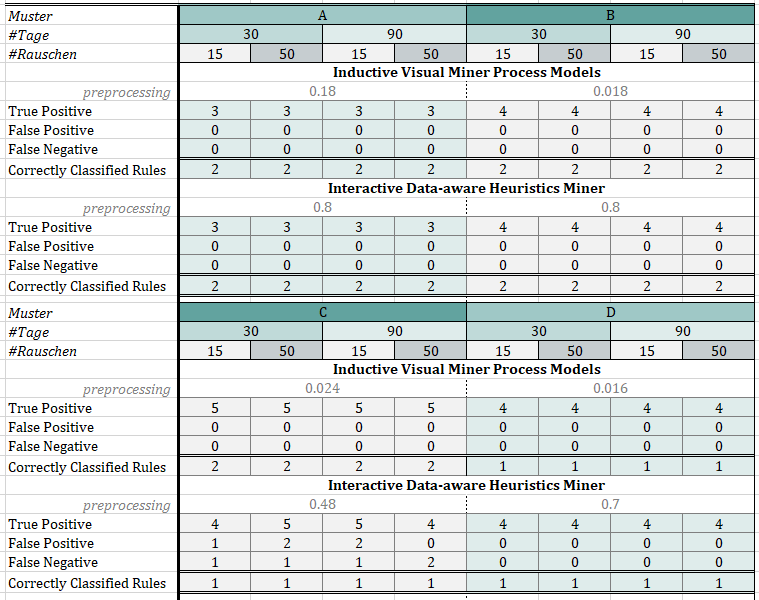
\includegraphics[width=0.9\textwidth]{figures/Appbildungen/tab1.PNG}
    \caption{Ergebnisse Versuchsreihe 'A' - 'D' des Inductive und Heuristic Miners}
    \label{tab1}
\end{figure}

\begin{figure}[!ht]
    \centering
    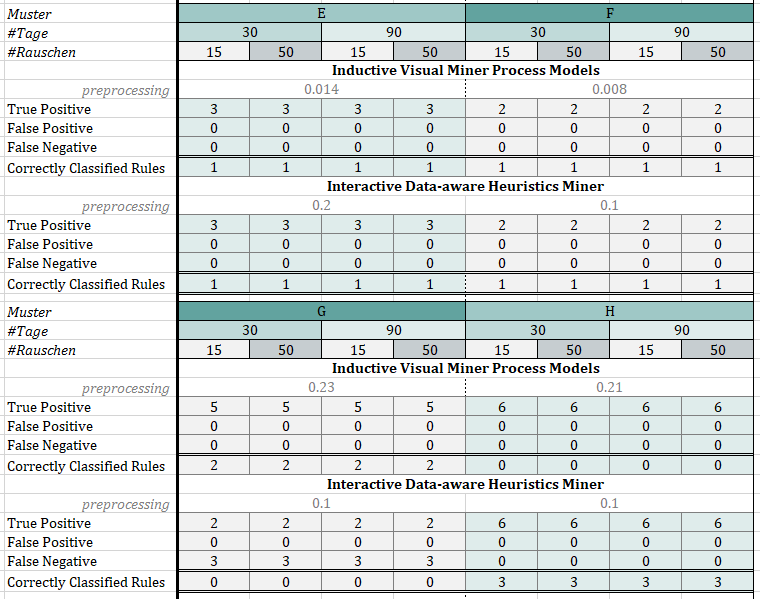
\includegraphics[width=\textwidth]{figures/Appbildungen/tab2.PNG}
    \caption{Ergebnisse Versuchsreihe 'E' - 'H' des Inductive und Heuristic Miners}
    \label{tab2}
\end{figure}

\begin{figure}[!ht]
    \centering
    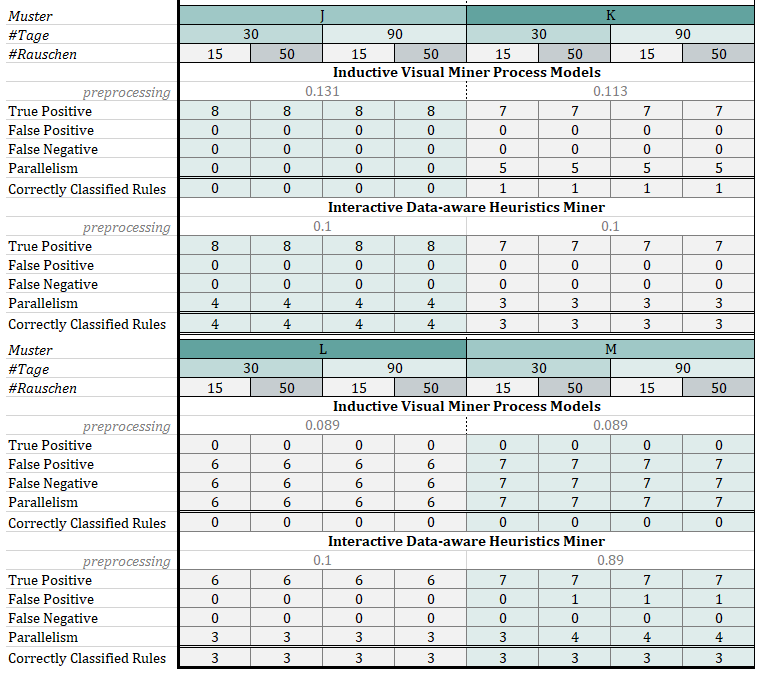
\includegraphics[width=\textwidth]{figures/Appbildungen/tab3.PNG}
    \caption{Ergebnisse Versuchsreihe 'J' - 'M' des Inductive und Heuristic Miners}
    \label{tab3}
\end{figure}

\clearpage
\subsubsection{Eventlogs generieren}\label{lst:generate}
\small
\begin{lstlisting}[language=Python]
import csv
import time
import random
import datetime as dt
from datetime import timedelta
#...
def addnoise(noise, casename, currenttimestamp):
    totalseconds_in_range = 5 * 60 * 60
    noisesum = int(( float(noise) / float(100.) ) * len(pattern_a)+len(pattern_b))
    for i in range(noise):
        timestamp_noise_entry = currenttimestamp +dt.timedelta(seconds=random.randint(0,totalseconds_in_range))
        randNoiseEntrance = random.randint(0,(len(pattern_n)-1))
        eventlog.append([casename, str(timestamp_noise_entry), pattern_n[randNoiseEntrance][0],  pattern_n[randNoiseEntrance][0]+" "+pattern_n[randNoiseEntrance][1]])
        
def eventlogfill():
    var_case = 'A'
    var_case_ext = 'A'
    v = var_case_ext+var_case
    for i in range(days):
        minutes_diff = 30
        timestamp_it = timestamp_start + dt.timedelta(days=i)
        timestamp_it_end = timestamp_it + dt.timedelta(hours=5)
        totalseconds_in_range = 5 * 60 * 60
        
        addnoise(noise, v,timestamp_it)
        randsec = random.randint(5,55)
    
        if (i) % 10 == 0:
            #i
            timestamp_it_one = timestamp_it + dt.timedelta(minutes=(minutes_diff))
            eventlog.append([str(v), str(timestamp_it_one), rule_X_i[0],  
                                        rule_X_i[1]])
            timestamp_it_one_b = timestamp_it_one+ dt.timedelta(seconds=80+3*randsec)
            eventlog.append([str(v), str(timestamp_it_one_b),  rule_X_ii[0],  
                                        rule_X_ii[1]])
            #ii
            timestamp_it_two = timestamp_it_one_b + dt.timedelta(minutes=(minutes_diff))            
            eventlog.append([str(v), str(timestamp_it_two), rule_Y_i[0],  
                                       rule_Y_i[1]])
            timestamp_it_two_b = timestamp_it_two+ dt.timedelta(seconds=80+3*randsec)        
            eventlog.append([str(v), str(timestamp_it_two_b), rule_Y_ii[0],  
                                        rule_Y_ii[1]])
            #iii
            timestamp_it_three = timestamp_it_two_b + dt.timedelta(minutes=(minutes_diff))        
            eventlog.append([str(v), str(timestamp_it_three),  rule_Z_i[0],  
                                        rule_Z_i[1]])
            timestamp_it_three_b = timestamp_it_three+ dt.timedelta(seconds=80+3*randsec)
            eventlog.append([str(v), str(timestamp_it_three_b),  rule_Z_ii[0],  
                                        rule_Z_ii[1]])
            timestamp_it_three_c = timestamp_it_three_b+ dt.timedelta(seconds=80+3*randsec)
            eventlog.append([str(v), str(timestamp_it_three_c),  rule_Z_iii[0],  
                                        rule_Z_iii[1]])
        #...
        v = var_case_ext+var_case+""
        
        if ord(var_case)>=90:
            var_case = 'A'
            var_case_ext = chr(ord(var_case_ext) + 1)
        else:
            var_case = chr(ord(var_case) + 1)
    eventlog.sort(key=lambda events: events[1])

def createcsv():
    with open('...\\CSVtoXES\\NAME\\IN\\'+filename+'.csv', 'w', newline='') as csvfile:
            filewriter = csv.writer(csvfile, delimiter=',', quotechar='|', quoting=csv.QUOTE_MINIMAL)
            filewriter.writerow(['case', 'timestamp', 'resource', 'activity'])
            for i in range(len(eventlog)):
                filewriter.writerow(eventlog[i])
    print("writing completed")

eventlogfill()
createcsv()
\end{lstlisting}

\clearpage
\subsubsection{Eventlogs nach XES Parsen}
\begin{lstlisting}[language=Python]
def generateXes(NDUI):
    records = []
    f = open(OUTdirectory+NDUI+".xes", "w+")
  
    iterlines = iter(csvfile)
    next(iterlines)
    for line in csvfile:
        parts = line.split(',')
        case = parts[0]
        timestamp = parts[1]
        resource = parts[2]
        activity = parts[3].rstrip()
    
        datetime_object = datetime.strptime(timestamp, '%Y-%m-%d %H:%M:%S')
    
        record = {"case":case, "timestamp":datetime_object, "resource":resource, "activity":activity}
        records.append(record)
    csvfile.close()
    
    header = """<?xml version="1.0" encoding="UTF-8" ?>
    <!-- This file has been generated with the OpenXES library. It conforms -->
    <!-- to the XML serialization of the XES standard for log storage and -->
    <!-- management. -->
    <!-- XES standard version: 1.0 -->
    <!-- OpenXES library version: 1.0RC7 -->
    <!-- OpenXES is available from http://www.openxes.org/ -->
    <log xes.version="1.0" xes.features="nested-attributes" openxes.version="1.0RC7">
    	<extension name="Lifecycle" prefix="lifecycle" uri="http://www.xes-standard.org/lifecycle.xesext"/>
    	<extension name="Time" prefix="time" uri="http://www.xes-standard.org/time.xesext"/>
    	<extension name="Concept" prefix="concept" uri="http://www.xes-standard.org/concept.xesext"/>
    	<classifier name="Event Name" keys="concept:name"/>
    	<classifier name="(Event Name AND Lifecycle transition)" keys="concept:name lifecycle:transition"/>
    	<string key="concept:name" value="XES Event Log"/>"""
    footer = "</log>"
    
    f.write(header)
    currentday=None
    currentmonth=None
    currentyear=None
    id = 100
    for record in records:
        if currentday is None:
            f.write('\t<trace>\n')
            currentday = record['timestamp'].day
            currentmonth= record['timestamp'].month
            currentyear= record['timestamp'].year
            case = record['case']
            print(str(case))
            f.write('\t\t<string key="concept:name" value="'+case+'"/>\n')
        else:
            if currentday != record['timestamp'].day or currentmonth != record['timestamp'].month or currentyear != record['timestamp'].year:
                f.write('\t</trace>\n')
                f.write('\t<trace>\n')
                case = record['case']
                print(str(case))
                f.write('\t\t<string key="concept:name" value="'+case+'"/>\n')
                #case = chr(ord(case)+1)
                currentday = record['timestamp'].day
                currentmonth= record['timestamp'].month
                currentyear= record['timestamp'].year
        f.write('\t\t<event>\n')
        f.write('\t\t\t<string key="resource" value="'+record['resource']+'"/>\n')
        f.write('\t\t\t<string key="lifecycle:transition" value="start"/>\n')
        f.write('\t\t\t<string key="concept:name" value="'+record['activity']+'"/>\n')
        datestring = record['timestamp'].strftime('%Y-%m-%dT%H:%M:%S.000+02:00')
        f.write('\t\t\t<date key="time:timestamp" value="'+datestring+'"/>\n')
        f.write('\t\t\t<int key="Event ID" value="'+str(id)+'"/>\n')
        id +=1
        f.write('\t\t</event>\n')
    
    f.write('\t</trace>')    
    f.write(footer)

for filename in os.listdir(directory):
    if(filename.endswith('.csv')):
        csvfile=open(os.path.join(directory, filename), 'r')
        print(filename)
        generateXes(filename)
    else:
        continue

\end{lstlisting}

\clearpage
\subsubsection{Konfiguration der Versuchsreihen}\label{sec:config}
Eingabedaten für den Eventloggenerator.
Je Versuchsreihe wurden vier Eventlogs generiert, die jeweils Zeilen der Schemata 'A' - 'M' enthielten.
\begin{table}[!ht]
\centering
\resizebox*{!}{0.8\textheight}{%
\begin{tabular}{llll}
\hline
\textbf{Bez.} & \textbf{Resource}             & \textbf{Activity}                         & \textbf{About}            \\ \hline
A             & \textit{}                     & \textit{}                                 & Rules                     \\
i             & \textit{Doorbell}             & \textit{ringing}                          & \multicolumn{1}{r}{2}     \\
ii            & \textit{Coffee Maker}         & \textit{turned to ON}                     & Nodes                     \\
              & \textit{Coffee Maker}         & \textit{Two Esprosso Cups}                & \multicolumn{1}{r}{3}     \\ \hline
B             & \textit{}                     & \textit{}                                 & Rules                     \\
i             & \textit{Coffee Maker}         & \textit{turned to ON}                     & \multicolumn{1}{r}{2}     \\
              & \textit{Coffee Maker}         & \textit{Two Esprosso Cups}                & Nodes                     \\
ii            & \textit{Doorbell}             & \textit{recognized a face (registered)}   & \multicolumn{1}{r}{4}     \\
              & \textit{Doorbell}             & \textit{ringing}                          &                           \\ \hline
C             & \textit{}                     & \textit{}                                 & Rules                     \\
i             & \textit{Alarm}                & \textit{turned on}                        & \multicolumn{1}{r}{2}     \\
              & \textit{Bathroom Light}       & \textit{set to ON}                        & Nodes                     \\
              & \textit{Bathroom Light}       & \textit{set to OFF}                       & \multicolumn{1}{r}{5}     \\
ii            & \textit{Coffee Maker}         & \textit{Two Esprosso Cups}                &                           \\
              & \textit{Coffee Maker}         & \textit{set to OFF}                       &                           \\ \hline
D             & \textit{}                     & \textit{}                                 & Rules                     \\
i             & \textit{Garage Door}          & \textit{Garage Door opened}               & \multicolumn{1}{r}{1}     \\
              & \textit{Garage Door}          & \textit{Garage Door closed}               & Nodes                     \\
              & \textit{smartlight 02}        & \textit{switched to ON}                   & \multicolumn{1}{r}{4}     \\
              & \textit{smartlight 02}        & \textit{switched to OFF}                  &                           \\ \hline
E             & \textit{}                     & \textit{}                                 & Rules                     \\
i             & \textit{smartlight main}      & \textit{turned to ON}                     & \multicolumn{1}{r}{1}     \\
              & \textit{weather sensor}       & \textit{currently snowing}                & Nodes                     \\
              & \textit{heating element}      & \textit{turned to ON}                     & \multicolumn{1}{r}{3}     \\ \hline
F             & \textit{}                     & \textit{}                                 & Rules                     \\
i             & \textit{front door}           & \textit{unlocked}                         & \multicolumn{1}{r}{1}     \\
              & \textit{smartlight 02}        & \textit{turned to on}                     & Nodes                   2 \\ \hline
G             & \textit{}                     & \textit{}                                 & Rules                     \\
i             & \textit{Garage Door}          & \textit{opened}                           & \multicolumn{1}{r}{2}     \\
              & \textit{Garage Door}          & \textit{closed}                           & Nodes                     \\
              & \textit{smartlight 02}        & \textit{switched to ON}                   & \multicolumn{1}{r}{7}     \\
              & \textit{smartlight 02}        & \textit{switched to OFF}                  &                           \\
ii            & \textit{Alarm}                & \textit{turned on}                        &                           \\
              & \textit{Bathroom Light}       & \textit{set to ON}                        &                           \\
              & \textit{Bathroom Light}       & \textit{set to OFF}                       &                           \\ \hline

\end{tabular}%
}
\caption{Konfiguration Versuchsreihe 'A' - 'G'}
\label{tab:Versuchskonfig1}
\end{table}

\clearpage
\begin{table}[]
\centering
\resizebox{\textwidth}{!}{%
\begin{tabular}{llll}
\hline
\textbf{Bez.} & \textbf{Resource}             & \textbf{Activity}                         & \textbf{About}            \\ \hline
H             & \textit{}                     & \textit{}                                 & Rules                     \\
i             & \textit{Smart TV}             & \textit{turned to ON}                     & \multicolumn{1}{r}{3}     \\
              & \textit{Smart TV}             & \textit{switched to CHANNEL 1}            & Nodes                     \\
ii            & \textit{Smart Alarm Clock}    & \textit{turned to ON}                     & \multicolumn{1}{r}{6}     \\
              & \textit{CLEVER Coffee Maker}  & \textit{two Espresso Cups}                &                           \\
iii           & \textit{Nested Thermostat}    & \textit{SET TO 18 DEG}                    &                           \\
              & \textit{Light Fixture}        & \textit{turned to ON}                     &                           \\ \hline
J             & \textit{}                     & \textit{}                                 & Rules                     \\
i             & \textit{Smart TV}             & \textit{turned to ON}                     & \multicolumn{1}{r}{4}     \\
              & \textit{Smart TV}             & \textit{switched to CHANNEL 1}            & Nodes                     \\
ii            & \textit{Smart Alarm Clock}    & \textit{turned to ON}                     & \multicolumn{1}{r}{8}     \\
              & \textit{CLEVER Coffee Maker}  & \textit{two Espresso Cups}                &                           \\
iii           & \textit{Nested Thermostat}    & \textit{SET TO 18 DEG}                    &                           \\
              & \textit{Light Fixture}        & \textit{turned to ON}                     &                           \\
iv            & \textit{Light Fixture}        & \textit{turned to OFF}                    &                           \\
              & \textit{Nested Thermostat}    & \textit{SET TO 13 DEG}                    &                           \\ \hline
K             & \textit{}                     & \textit{}                                 & Rules                     \\
i             & \textit{Smart TV}             & \textit{turned to ON}                     & \multicolumn{1}{r}{3}     \\
              & \textit{Smart TV}             & \textit{switched to CHANNEL 1}            & Nodes                     \\
              & \textit{Smart TV}             & \textit{set Volume to 22}                 & \multicolumn{1}{r}{7}     \\
ii            & \textit{Smart Alarm Clock}    & \textit{turned to ON}                     &                           \\
              & \textit{CLEVER Coffee Maker}  & \textit{two Espresso Cups}                &                           \\
iii           & \textit{Nested Thermostat}    & \textit{SET TO 18 DEG}                    &                           \\
              & \textit{Light Fixture}        & \textit{turned to ON}                     &                           \\ \hline
L*            & \textit{}                     & \textit{}                                 & Rules                     \\
i             & \textit{Smart TV}             & \textit{turned to ON}                     & \multicolumn{1}{r}{3}     \\
              & \textit{Smart TV}             & \textit{switched to Streaming Service TM} & Nodes                     \\
ii            & \textit{Smart Alarm Clock}    & \textit{turned to ON}                     & \multicolumn{1}{r}{6}     \\
              & \textit{CLEVER Coffee Maker}  & \textit{two Espresso Cups}                &                           \\
iii           & \textit{Garage Door}          & \textit{Light turned Off}                 & *every other day          \\
              & \textit{Garage Door}          & \textit{Door closed}                      &                           \\ \hline
M*            & \textit{}                     & \textit{}                                 & Rules                     \\
i             & \textit{Smart TV}             & \textit{turned to ON}                     & \multicolumn{1}{r}{3}     \\
              & \textit{Smart TV}             & \textit{switched to Streaming Service TM} & Nodes                     \\
ii            & \textit{Garage Door}          & \textit{Light turned Off}                 & \multicolumn{1}{r}{7}     \\
              & \textit{Garage Door}          & \textit{Door closed}                      &                           \\
iii           & \textit{Nested Thermostat}    & \textit{SET TO 16 DEG}                    & *every third day          \\
              & \textit{Main Light}           & \textit{turned to OFF}                    &                           \\
              & \textit{Floor Heating System} & \textit{turned to OFF}                    &                           \\ \hline
			  \end{tabular}%
}
\caption{Konfiguration Versuchsreihe 'H' - 'M'}
\label{tab:Versuchskonfig2}
\end{table}



\clearpage
\subsubsection{Hausautomatisierung durch Regelerkennung}\small
\begin{lstlisting}[language=Java]
public class PMFirebaseMessagingService extends FirebaseMessagingService {

    static String TAG = "ProcessMining MessagingService";
    static String currentToken = "";

    /**
     * Called if InstanceID token is updated. This may occur if the security of
     * the previous token had been compromised. Note that this is called when the InstanceID token
     * is initially generated so this is where you would retrieve the token.
     */
    @Override
    public void onNewToken(String token)
    {
        Log.d(TAG, "Refreshed token: " + token);

        // If you want to send messages to this application instance or
        // manage this apps subscriptions on the server side, send the
        // Instance ID token to your app server.
        currentToken = token;
    }

    public static void refreshID()
    {
        FirebaseInstanceId.getInstance().getInstanceId()
                .addOnCompleteListener(new OnCompleteListener<InstanceIdResult>() {
                    @Override
                    public void onComplete(@NonNull Task<InstanceIdResult> task) {
                        if (!task.isSuccessful()) {
                            //To do//
                            return;
                        }
                        // Get the Instance ID token//
                        String token = task.getResult().getToken();
                        PMFirebaseMessagingService.currentToken = token;
                        Log.d(TAG, "Got Firebase ID: " + token);
                    }
                });

        FirebaseMessaging.getInstance().subscribeToTopic("rules")
                .addOnCompleteListener(new OnCompleteListener<Void>() {
                    @Override
                    public void onComplete(@NonNull Task<Void> task) {

                        if (!task.isSuccessful()) {
                            Log.d(TAG, "Sub to topic not success");
                        }
                        Log.d(TAG, "Sub to topic success");
                    }
                });
    }

    @Override
    public void onMessageReceived(RemoteMessage remoteMessage)
    {
        super.onMessageReceived(remoteMessage);
        String newRules = "";
        for(String key : remoteMessage.getData().keySet())
            Log.d(TAG, "onMessageReceived: got key: " + key);

        if(remoteMessage.getData().containsKey("newRules"))
            newRules = remoteMessage.getData().get("newRules");

        Log.d("onMessreceived","got a message: "+newRules);
        PowerManager pm = (PowerManager) this.getSystemService(Context.POWER_SERVICE);
        boolean isScreenOn = pm.isScreenOn();
        Log.e("screen on.................................", "" + isScreenOn);
        if (isScreenOn == false)
        {
            @SuppressLint("InvalidWakeLockTag") PowerManager.WakeLock wl = pm.newWakeLock(PowerManager.FULL_WAKE_LOCK | PowerManager.ACQUIRE_CAUSES_WAKEUP | PowerManager.ON_AFTER_RELEASE, "MyLock");
            wl.acquire(10000);
            @SuppressLint("InvalidWakeLockTag") PowerManager.WakeLock wl_cpu = pm.newWakeLock(PowerManager.PARTIAL_WAKE_LOCK, "MyCpuLock");

            wl_cpu.acquire(10000);

        }
           startActivity(new Intent(this, MainActivity.class));

        Log.d(TAG, "onMessageReceived: " + remoteMessage.getData().get("message") + " to: " + remoteMessage.getTo());

        Intent intent = new Intent(this, PMRulesTabs.class);
        intent.addFlags(Intent.FLAG_ACTIVITY_CLEAR_TOP);
        PendingIntent pendingIntent = PendingIntent.getActivity(this, 0, intent, PendingIntent.FLAG_ONE_SHOT);

        String channelId = "Default";
        NotificationCompat.Builder builder = new  NotificationCompat.Builder(this, channelId)
                .setSmallIcon(R.mipmap.ic_launcher)
                .setContentTitle("PM")
                .setContentText("new suggested rule received!").setAutoCancel(true).setContentIntent(pendingIntent);;
        NotificationManager manager = (NotificationManager) getSystemService(NOTIFICATION_SERVICE);
        if (Build.VERSION.SDK_INT >= Build.VERSION_CODES.O) {
            NotificationChannel channel = new NotificationChannel(channelId, "Default channel", NotificationManager.IMPORTANCE_HIGH);
            manager.createNotificationChannel(channel);
        }
        manager.notify(0, builder.build());

        try {
            parseReceivedRule(newRules);
        } catch (JSONException e) {
            e.printStackTrace();
        }
    }

    private void parseReceivedRule(String newRule) throws JSONException {
        JSONArray allNodes = new JSONArray(newRule);
        Log.d("process", "All Rules: "+allNodes.getJSONArray(0)+ " 1: "+allNodes.getJSONArray(1));
        for (int i = 0; i < allNodes.length(); i++) {
            try {
                // JSONObject node = rules.getJSONObject(i);
                JSONArray rule = allNodes.getJSONArray(i);
                Log.d("process", "rule: "+i+". "+rule);
                PMRule.processRule(rule);
            } catch (JSONException e) {
                Log.d("process", "Json exception: "+e);
            }
        }
    }
\end{lstlisting}
\normalsize

\fancyhead[RE,RO]{Literaturverzeichnis}

    % bibliography is not in the table of contents per default, add it manually
    \addcontentsline{toc}{chapter}{Literaturverzeichnis}

    \bibliographystyle{ieeetr}
    \bibliography{bib/topic1}
    \newpage
    \thispagestyle{empty}
    \mbox{}
    

\end{document}